\chapter{隐私保护外包K-means聚类技术研究}

\section{引言}
%搬运开题报告
%随着现代社会数字化的不断演进,数据使用量呈指数级增加,个人和小型组织越来越难以在内部计算机服务器上维护所有重要信息、运行大型程序和系统。为解决这些问题,云计算应运而生。自云计算在2006年被提出后,它就被认为是能够推动下一代互联网革命的技术,并迅速成为了研究领域的热门话题\cite{sadiku2014cloud}。近年来,随着研究的发展和设备的进步,机器学习从学术研究落地到生活的方方面面,但是大多数机器学习任务对于设备的性能要求较高,需要存储海量的数据才能取得较好的结果。大型公司有能力承担设备费用,利用机器学习的便利开展各种各样的服务,但是资源受限的小公司和个人的需求常常难以被满足。
%
%为解决上述问题,云计算场景下出现了一种新的服务类型-MLaaS,即“机器学习即服务(Machine Learning as a Service)”,它使得技术可以扩展,并且价格合理\cite{ribeiro2015mlaas}。在MLaaS中,海量的数据需要被上传到云计算中心,这一过程也被称之为外包计算。由于用户在数据上传后失去了对数据的完全控制,因此会更加关心隐私安全问题。同时云计算服务模型的复杂性、实时性,数据的多元异构特点以及终端资源有限,传统的数据安全隐私和隐私保护方法无法直接用来保护云计算中的大量数据\cite{hunt2018chiron}。
%
%聚类(Clustering)是一种非常流行的无监督机器学习技术,它了能够将相似的输入元素划分到同一个簇(cluster)中。聚类的应用领域非常广泛,从业务分析到医疗保健等诸多领域。在许多这些应用场景中,敏感信息在被正确聚类的同时,也不应该被泄漏。此外,现在经常需要将不同来源的数据组合起来进行训练以提升分析质量,庞大的数据量对资源受限的用户带来巨大的压力,因此,通常需要将复杂的计算外包给强大的云服务器进行处理,这就要求我们设计有效隐私保护聚类方案\cite{ahmed2020k}。
%
%目前,为了保护聚类过程中输入的敏感数据的隐私,已经有了许多研究成果,涵盖各个方面。在设计隐私保护聚类协议时,通常考虑两个不同的场景。在多方计算的场景下\cite{cramer2015secure},两个及两个以上的数据所有者共同执行安全计算协议,除了输出之外的任何内容都不会泄漏给彼此,比较常见的是两方计算。同时,一些研究也会在模型设计中引入半诚实参与方(通常是服务器)来辅助计算。相对应的,另一种场景则是外包计算\cite{li2018privacy},一个或多个数据所有者将将计算(或存储)外包给其他参与方,我们假设这些参与方可以为数据所有者进行聚类而无需知道关于输入数据的任何信息。由于外包计算旨在使用外部资源,数据所有者通常不应该参与协议的执行,处于离线状态,但是这一点通常难以完全实现。值得一提的是,一些多方计算(MPC)议也可以用于外包计算场景,只需要数据所有者在多个不共谋的参与方之间秘密共享自己的数据,然后多个参与方在秘密共享的数据上执行聚类算法。但是,MPC协议是否支持外包计算很大程度上取决于协议设计,如果数据持有者需要在聚类过程中进行大量的明文计算或者在中间对数据进行解密,那就很难将协议转换到外包计算的场景。
%
%外包计算和多方计算都各有其优势,但是对于资源受限的用户来说,外包计算则更加具有实际意义,基于外包计算的安全计算方法已有诸多研究,但是完全安全的聚类方案通常效率较低,即便是在性能较好的服务器上也需要花费难以接受的时间才能获得最终结果,效率较高的方案通常会牺牲一定的安全性,泄漏中间计算结果,例如簇大小,簇中心,这些都会导致一些隐私安全问题。因此如何设计出安全又高效的外包聚类方案值得深入研究和探索。
%
%针对上述研究现状,我们研究在外包计算场景下,如何在保护用户隐私数据和聚类中间结果以及保证效率可接受的同时,精确的完成聚类计算。首先,我们选择应用最为广泛的K-means聚类方案。K-means聚类是最简单和流行的无监督学习算法之一,能够应用于大型数据集,并且具有良好的收敛性。其次,我们引入Kd-tree来加速聚类过程,Kd-tree是一种空间划分数据结构,将空间上靠近的数据放在同一个节点中,广泛用于空间相关应用来加速计算。基于此,我们提出了一种基于Kd-tree的隐私保护K-means聚类方法。方案由客户端和双云服务器参与,用户在本地明文基础上构造Kd-tree,然后秘密共享所有数据分别发送给双云,云服务器在密文基础上运行系列安全协议来获取聚类结果后,将密文结果发送给用户,用户进行还原。理论分析与实验验证表明,方案在为用户提供外包聚类计算的同时,保证了数据的安全性,计算的高效性以及聚类结果的精确性。
%
%本章的组织结构如下:第\ref{s3-yubei}节介绍了安全性定义、基于Kd-tree的K-means聚类以及基于秘密共享的安全多方计算。第\ref{s3-wenti}节中描述了系统模型、安全模型以及设计目标。第\ref{s3-mokuai}节中提出了一系列基于秘密共享的隐私保护计算模块。第\ref{s3-ppokc}节中提出了基于Kd-tree的隐私保护K-means聚类方案。第\ref{s3-lilun}从理论上分析了方案的正确性和安全性。第\ref{s3-shiyan}节中对方案进行了全面的实验评估。最后,在\ref{s3-xiaojie}节中对本章进行了总结。

K-means聚类是一种广泛应用的无监督机器学习算法,能够将相似的输入元素划分到同一个簇中,使不同簇之间的差异尽可能大,它的应用领域非常广泛,从业务分析,市场营销到医疗数据处理等等。随着现代社会数字化的不断演进,数据使用量呈指数级增加趋势,资源有限的独立用户与小型组织越来越难以在内部计算机系统上对大量数据进行聚类分析。同时,随着研究的深入,提升聚类算法的效果要求联合多个来源的数据进行训练,这也给传统的聚类模式带来了挑战。

云计算提供的机器学习即服务能够较好的解决上述问题,它为用户提供资源和服务来运行机器学习算法,允许多方上传数据并且价格合理方便快捷\cite{ribeiro2015mlaas}。在MLaaS中,海量的数据需要被上传到云计算中心,这也带来了新的挑战。一方面,聚类所用数据可能包含敏感信息,直接将数据交给云平台进行聚类会带来潜在的隐私信息泄露风险;另一方面,在加密的数据上进行隐私保护聚类可能会导致耗时较长,计算与通信开销较大,使数据的可用性降低。

目前,云环境下的隐私保护外包K-means聚类方案已经有了较多研究成果\cite{mohassel2019practical,wu2020secure,rong2017privacy,jaschke2019unsupervised},Mohassel等人\cite{mohassel2019practical}基于混淆电路、不经意传输以及秘密共享提出了一种安全高效的K-means聚类方案,但是该方案通信开销巨大,要求云服务器进行多轮交互。Wu等人\cite{wu2020secure}基于能够进行密文打包的同态加密方案提出了一种外包K-means聚类方案,结合K-means聚类中计算的特点,对密文进行并行计算以获取最终结果,虽然该方案显著提升了隐私保护聚类方案的效率,缩短了耗时,但是中间协议泄露了数据分布特点,存在安全隐患。

针对上述研究现状,本文研究在外包计算场景下,如何在保护用户隐私数据和聚类中间结果以及保证效率可接受的同时,精确的完成K-means计算。首先,引入Kd-tree来加速聚类过程,Kd-tree是一种空间划分数据结构,将空间上靠近的数据放在同一个节点中,广泛用于空间相关应用来加速计算。基于此,本文提出了一种基于Kd-tree的隐私保护K-means聚类方法。方案由独立用户和双云服务器参与,用户在本地明文基础上构造Kd-tree,然后秘密共享所有数据分别发送给双云,云服务器在密文基础上运行系列安全协议来获取聚类结果后,将密文结果发送给用户,用户进行还原。

本章的组织结构如下:第\ref{s3-yubei}节介绍了安全性定义、基于Kd-tree的K-means聚类以及基于秘密共享的安全多方计算。第\ref{s3-wenti}节中描述了系统模型、安全模型以及设计目标。第\ref{s3-mokuai}节中提出了一系列基于秘密共享的隐私保护计算模块。第\ref{s3-ppokc}节中提出了基于Kd-tree的隐私保护K-means聚类方案。第\ref{s3-lilun}节从理论上分析了方案的正确性和安全性。第\ref{s3-shiyan}节中对方案进行了全面的实验评估。最后,在\ref{s3-xiaojie}节中对本章进行了总结。
\section{预备知识}
\label{s3-yubei}
\subsection{半诚实模型}
\label{s3-anquanmoxing}
半诚实模型(Semi-honest Model),也称为诚实且好奇的模型(Honest-but-curious Model),指的是参与方会诚实的执行所有协议,但会竭尽所能利用已有的信息获取尽可能多的内容。半诚实的参与方通常是被动的,因为他们除了通过观察执行协议的过程无法采取其他任何行动来获取隐私数据。这样的模型广泛应用于诸多研究来支持密文数据上交互协议的研究。具体定义\cite{oded2009foundations}如\ref{defi-semihonest}所示:

\begin{definition}
	\label{defi-semihonest}
	假设参与方$ C_i $的输入为$ x_i $,对于任意协议$ \pi $,$ C_i $的执行镜像为$\Pi_{\mathrm{i}}(\pi)$,并且$ C_i $根据协议$ \pi $的计算输出为$ y_i$。若可以根据$ x_i $和$ y_i $模拟$\Pi_{\mathrm{i}}(\pi)$,且它的模拟镜像分布与实际执行镜像分布计算不可区分(Computationally Indistinguishable),则可以认为$ \pi $是安全的。
\end{definition}

\subsection{基于Kd-tree的K-means聚类方法}
K-means聚类是最常用的聚类算法之一,给定簇个数$ k $,它能够将大小为$ n $的数据集划分成$ k $个内容不相交的子集。每个簇都有一个中心点,对单个数据而言,该数据点到最终所属簇中心的距离相较于其他簇更短。K-means聚类算法有多种不同的实现方式,以使聚类更加高效便捷。论文\cite{kanungo2002efficient}的核心思想是以Kd-tree为主要数据结构,设计了一种高效的过滤算法来聚类数据。

\subsubsection{Kd-tree数据结构}
Kd-tree是一种空间划分数据结构,将空间上靠近的点划分到树的同一个节点中\cite{el2020kd},通常应用于加速与点空间相关的计算,例如k近邻算法和创建点云。

这里,本文遵循如下规则来创建Kd-tree:
\begin{compactitem}
	\item 在$ k$维数据集中,计算数据每个维度的方差,选择方差最大的维度$ d_{max} $来划分数据
	\item 找到$ d_{max} $维度数据的中位数$ m $作为基准来划分数据集,得到两个子集合
	\item 对划分出的子集重复上述过程直到Kd-tree构造完成
\end{compactitem}

Kd-tree数据结构有两个主要的优势,一方面,它能够将可能属于同一个数据集的点划分到同一个树节点中。另一方面,它采取一种高效的方式来将初始空间划分为两个子空间以加速后续数据处理。

\subsubsection{过滤算法}
\label{s3-guolvsuanfa}
本小节详细介绍论文\cite{kanungo2002efficient}的核心,过滤算法。给定$ n $个点,构造的Kd-tree包含$ O(n) $个节点,高度为$ O(\log n) $。对于Kd-tree中每个节点$ u $,计算包含的数据个数$ u.count $以及加权质心$ u.wgtCent $,即包含点数据之和。中心的计算方式为$ u.wgtCent/u.count $,在构造Kd-tree的过程中可以连带计算上述内容。初始簇中心采取从数据集中随机选择的方式。
\begin{algorithm}[htbp]
	\renewcommand{\algorithmicrequire}{\textbf{输入:}}
	\renewcommand{\algorithmicensure}{\textbf{输出:}}
	\caption{过滤算法}
	\label{alg_filter}
	\begin{algorithmic}[1]
		\REQUIRE Kd-tree节点$u$,候选集合$Z$
		\ENSURE 聚类后的簇
		\STATE $C \leftarrow u.cell$
		\IF{$u$为叶子节点}
		\STATE $z^{*}$为Z中距离点u最近的簇
		\STATE $z^{*}.wgtCent \leftarrow z^{*}.wgtCent + u.point$
		\STATE $ z^{*}.count \leftarrow z^{*}.count + 1 $
		\ELSE
		\STATE $ z^* $为Z中距离u的中心点最近的簇
		\FOR{each $ z $ in $Z \backslash \{z^*\}$}
		\IF{$ z.isFarther(z^*, C) $}
		\STATE $ Z \leftarrow Z \backslash \{z\} $
		\ENDIF
		\ENDFOR
		\IF{$ |Z| = 1 $}
		\STATE $ z^*.wgtCent\leftarrow z^*.wgtCent+u.wgtCent$
		\STATE $z^*.count\leftarrow z^*.count+u.count$
		\ELSE
		\STATE Filter(u.left, Z)
		\STATE Filter(u.right, Z)
		\ENDIF
		\ENDIF
	\end{algorithmic}
\end{algorithm}

对于Kd-tree中每个节点$ u $维护一个候选簇集合$ Z $,该集合中的簇均有可能为节点中所有数据的最终所属簇。对于根节点,候选簇为随机选择的$ k $个簇。按照算法\ref{alg_filter}中的方式来处理每个点的候选簇集合:对于每个节点$ u $,令$ C $为包含数据集合,$ Z $为候选簇集合。
若$ u $为叶子节点,则直接找到$ Z $中最近的候选簇$ z^* $,然后将该叶子节点内包含的数据划分到$ z^* $中。
若为Kd-tree中的非叶子节点,则需要进行更复杂的处理。首先计算$ C $的中心点,然后找到候选簇中距离中心最近的簇$ z^*\in Z $。
接下来,对比剩余的候选簇$ z\in Z\backslash\{z^*\} $,若$ C $中所有数据均距离$ z^* $更近,则认为$ z $不可能为节点$ u $中任何一个数据的最近所属簇,因此进行剪枝,即从候选簇中删除$ z $。
若经过上述处理,$ u $仅剩一个候选簇($ |Z|=1 $),即$ z^* $,则认为$ z^* $就是$ u $中所有数据的所属簇,可以将这些数据划分进$ z^* $中,并且将相关的$ u.wgtCent $和$ u.count $添加到$ z^* $中。否则,对其子节点重复上述过程。

一旦确定了节点中所有数据的最终所属簇,即可不用再对子节点进行处理,减少了冗余计算并提升聚类效率。Kd-tree数据结构的特点使得相似的数据点会被划分到同一个节点中,能够加速算法收敛。

\subsection{基于秘密共享的安全多方计算}
安全多方计算(SMPC)首先由\cite{yao1986generate}提出,它能够使多个参与方在不泄露自身输入数据的前提下协同进行计算获取结果,广泛用于各种隐私保护方案中。秘密共享是安全多方计算中一个常用工具,最早由Shamir\cite{rivest2001leak}和Blakley\cite{blakley1979safeguarding}于1979年分别提出。秘密共享的基本思路是:将秘密$ s $划分为$ n $份,分发给$ n $个不同的参与方,至少需要$ t $个不同的参与者才能够重构秘密,否则失败。接下来,本节以两个参与方$ A $与$ B $为例,详细介绍秘密共享相关计算。

假设所有数据的范围在环$ \mathbb{Z}_P $上,对于$ x $的加性秘密共享值$ \langle x \rangle $,有$ \langle x \rangle^A + \langle x \rangle^B = x\mod P$。参与方$ A $拥有$ \langle x \rangle^A $,参与方B同理。重构秘密$ x $($ Rec(\cdot, \cdot) $),其中一个参与方将分配给自己的秘密发送给另一方,然后计算$ x=\langle x\rangle^A+\langle x\rangle^B(\mod P) $。接下来的说明中,为了简化表示省略mod P说明。

\subsubsection{加性秘密共享加法}
为计算两个秘密共享值$ \langle x \rangle $($ \langle x \rangle^A,\langle x \rangle^B $)和$ \langle y \rangle $($ \langle y\rangle^A,\langle y\rangle^B $)之和,参与方$ A $与$ B $分别计算$\langle z\rangle^A=\langle x\rangle^A+\langle y\rangle^A$和$\langle z\rangle^B=\langle x\rangle^B+\langle y\rangle^B$。对于秘密共享值$ \langle x \rangle $与常量$ c $的加法,参与方$ A $在本地计算$\langle z\rangle^A=\langle x\rangle+c$,参与方$ B $计算$\langle z\rangle^B=\langle x\rangle^B$。
\subsubsection{秘密共享乘法}
秘密共享的安全乘法协议首先由Beaver\cite{beaver1992efficient}提出,为计算乘积$\langle z\rangle=\langle x\rangle \cdot\langle y\rangle$,需要一个预计算的乘法三元组$\langle c\rangle=\langle a\rangle \cdot\langle b\rangle$。其中参与方$ i $计算$ \langle e \rangle^i = \langle x \rangle^i - \langle a \rangle^i $和$\langle f\rangle^i=\langle y\rangle^i-\langle b\rangle^i$,其中$ i \in \{A, B\}$。参与方均运行$ Rec(\cdot, \cdot) $来恢复$ e $和$ f $。最后,参与方$ A $令$\langle z\rangle^A=f \cdot\langle a\rangle^A+e \cdot\langle b\rangle^A+\langle c\rangle^A$,参与方$ B $令$\langle z\rangle^B=e \cdot f+f \cdot\langle a\rangle^B+e \cdot\langle b\rangle^B+\langle c\rangle^B$,即计算完成。本文用MUL来表示乘法操作,若输入为两个秘密共享值,则输出对应乘法结果;若为两个秘密共享数组相乘,则输出对应元素相乘的秘密共享结果数组;若输入为多个秘密共享值,则输出为计算的多个数据连乘的结果。

值得注意的是,乘法主要分为两个阶段。离线阶段中,预计算的乘法三元组每次进行乘法时都要更新,但是三元组生成的过程是离线的,可以由两方通过不经意传输(Oblivious Transfer)生成\cite{schneider2013gmw},也可以由可信第三方提供\cite{riazi2018chameleon}。更多关于预计算乘法三元组的细节可以参考\cite{beaver1992efficient}。在线阶段中,两个参与方相互通信以获得最终的计算结果。
\section{问题描述}
\label{s3-wenti}

\subsection{系统与安全模型}
\begin{figure}[htbp]
	\centering
	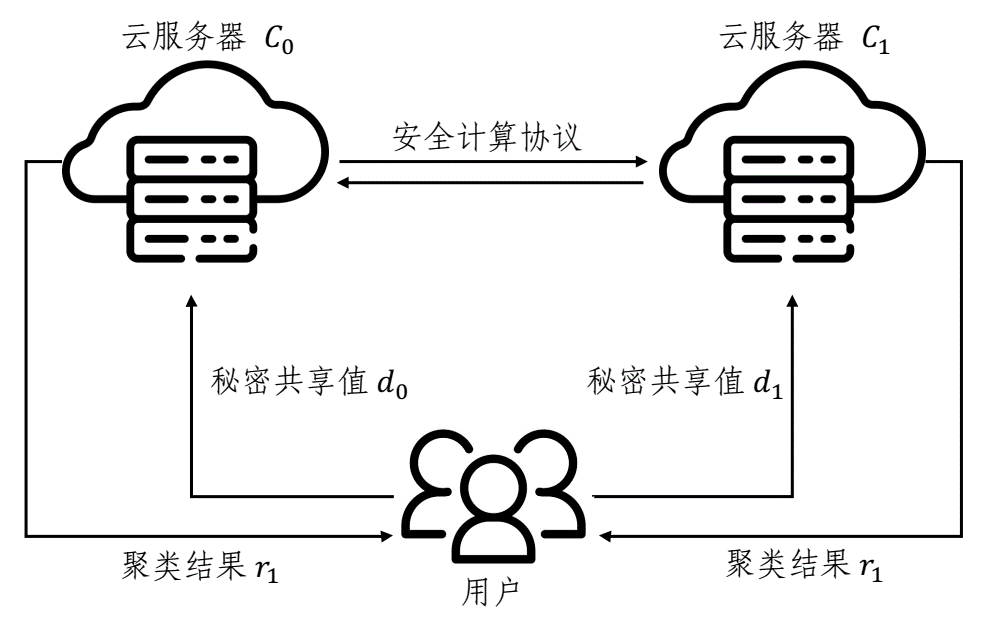
\includegraphics[width=0.75\linewidth]{img/sysmodel1.png}%width=\linewidth
	\caption{系统模型}
	\label{sys model}
\end{figure}

如图\ref{sys model}所示,本方案的系统由两个部分组成:用户和云服务器。这样的系统模型广泛用于隐私保护研究中\cite{wu2020secure,bunn2007secure}。这里的客户指的是,持有隐私数据需要聚类来进行数据分析和挖掘的独立用户,他们通常没有足够的计算资源来聚类海量数据,因此需要将计算任务外包以获取结果。常见的实际用户有医疗机构、金融机构等。服务器端通常指的是拥有大量计算资源,提供付费计算服务的云服务器运营厂商例如阿里云、腾讯云等,他们提供机器学习即服务(MLaaS)这一付费模式,用户上传数据后即可离线等待机器学习计算结果。下面详细介绍方案中的每一部分:

\begin{compactitem}
	\item \textbf{双云服务器}:在系统中有两个不共谋的云服务器,标识为$ C_0 $和$ C_1 $,而且均持有用户秘密共享后的数据。他们会在此基础上执行一系列安全协议来实现隐私保护K-means聚类,最后将秘密共享的结果发送给用户。
	\item \textbf{用户}:用户首先在原始数据上构造Kd-tree,然后选择随机数来将数据划分为两份秘密共享值,分别发送给双云服务器。在K-means聚类结束后,获取服务器返回的秘密共享结果,运行$ Rec(\cdot,\cdot) $来还原最终结果。
\end{compactitem}

这里,本文假定$C_0$和$C_1$为半诚实模型下不共谋的两个云服务器,在实际场景中,可以将这两个云服务器部署在不同的云服务提供商上,例如阿里云和腾讯云,为了公司各自的声誉和利益,二者可以做到保持相互独立不合谋,因此这里的假定可以在实际场景中实现。同时,两个云服务器为诚实但好奇的个体,意味着它们会如实的执行执行的协议,但也会企图通过各种不合谋的方式来推测感兴趣的隐私或敏感信息。
\subsection{设计目标}
本节所述隐私保护外包K-means聚类方案设计目标如下:
\begin{compactitem}
	\item \textbf{安全性}:所有外包数据例如中间计算结果、最终计算结果都不应泄露给双云服务器。同时,服务器无法从秘密共享值推断出原始数据内容以及相关数据特征,例如数据分布、距离大小关系等。
	\item \textbf{高效性}:方案应具备高效性,整个聚类过程主要由双云服务器进行,二者具有丰富的计算和通信资源,能够对海量数据进行处理,应当显著降低用户计算和通信开销。
	\item \textbf{正确性}:密文方案应不损失计算精度,例如距离计算结果不产生误差、中间协议的结果正确。双云服务器应当能够返回和明文聚类方案一致的计算结果。
\end{compactitem}
\section{基于秘密共享的隐私保护计算模块}
\label{s3-mokuai}
为了使用户与云端能够进行安全的交互,本文基于秘密共享技术设计了一系列基本的计算模块。用户通过产生随机值将明文数据拆分为两份密文发送给双云服务器,两方在秘密共享值的基础上进行系列计算和交互,获取最终结果。

\subsection{安全欧式距离计算协议}

计算簇$z$到点$x$之间的欧式距离的计算公式如下:
\begin{equation}
	\label{cal_dist}
	dist=\sqrt{\sum_{j=1}^m\left(z[j]-x[j]\right)^2}
\end{equation}

其中下标$j$标识数据的第$j$个维度,所有数据均为加性秘密共享值。在所有点均被划分到对应簇后,通过计算平均值获得簇的中心点。假设簇$z'_i$包含点个数为$|z'_i|$,包含的数据为${x_1,...,x_{|z'_i|}}$,那么簇$z'_i$的中心点计算方式如下:
\begin{equation}
	\label{cal_center}
	z_{i}^{\prime}[j]=\frac{x_{1}[j]+\cdots+x_{\left|z_{i}^{\prime}\right|}[j]}{\left|z_{i}^{\prime}\right|}=\frac{s_{i}^{\prime}[j]}{\left|z_{i}^{\prime}\right|}, 1 \leq j \leq m
\end{equation}

其中$s'_i[j]$表示簇$z'$中所有点第$j$个维度数据之和。在秘密共享值上进行除法比较困难,因此采用文献\cite{wu2020secure}中提到的放缩方法来将距离计算中的除法转变为乘法。首先,计算全局缩放因子$\alpha$以及簇$z_i$对应的$\alpha_i$,计算方式为:
\begin{equation}
	\label{cal_scale}
	\alpha=\prod_{j=1}^{k}\left|z_{j}\right|, \alpha_{i}=\prod_{j=1 \wedge i \neq j}^{k}\left|z_{j}\right|
\end{equation}

为了方便计算,省略公式\ref{cal_dist}中的根号计算,将整个公式改写为:
\begin{equation}
	\label{final_dist_eq}
	dist = \sum_{j=1}^{m}(\alpha x[j] - \alpha_{i}z_i[j])^2
\end{equation}

根据秘密共享方案的性质,可以针对公式\ref{final_dist_eq}做出改进,简化计算。在一轮迭代中,无论计算什么距离,缩放因子$\alpha$和$\alpha_i$的值以及相关的计算结果都是不变的,因此可以在每轮迭代开始计算这些固定值,减少后续冗余计算。同时,参数不相关的计算可以并行进行,减少云服务器交互的次数。

\subsection{安全比较协议}
\label{s3-securecomparison}
安全比较场景如下,参与方$p_i$拥有加性秘密共享值$\langle x_i \rangle$和$\langle y_i \rangle$,其中$i \in \{0, 1\}$,期望能够在不泄露$x$和$y$明文值的前提下,获取二者的大小关系$\delta = LT(x, y), \delta = \langle \delta \rangle_0 + \langle \delta \rangle_1$,其中$\delta = LT(x, y)$的具体含义如下:
\begin{equation}
	\operatorname{LT}(x, y)= \begin{cases}1, & \text { if } x<y \\ 0, & \text { if } x \geq y\end{cases}
\end{equation}

在文献\cite{rathee2020cryptflow2}中,作者提出了一个高效的安全比较协议来解决百万富翁问题,该方案能够同时比较多对数据,通信开销较小,计算复杂度低。经过多轮不经意传输(Oblivious Transfer)后,参与方$p_0$和$p_1$分别获得布尔秘密共享结果$\delta = LT(x, y) ,\delta = \langle \delta \rangle^B_0 \bigoplus \langle \delta \rangle^B_1$。

由于本研究中安全比较的输入与输出均为加性秘密共享值,本协议在上述百万富翁协议的基础上添加一些改进以构造安全比较协议。具体过程如算法\ref{alg_sc}所示:

百万富翁协议解决的是双方各自持有明文在不泄露自身数据的情况进行比较的问题,无法直接比较秘密共享值,因此这里进行如下改造,将秘密共享值之间的比较转换为明文上的比较。
首先,令云服务器$C_0$产生随机数$a,a\in\mathbb{Z}_n$,将秘密共享值$\langle x \rangle$与$\langle y\rangle$之间的比较转换为明文$a$与$x-y+a$之间的比较,若$x>y$,则$x-y+a>a$。上述转换只需要一轮交互即可完成,通信和计算开销均较小。

针对协议的输出,需要将布尔秘密共享值($v=\langle v\rangle^B_0 \bigoplus \langle v\rangle^B_1$)转变为加性秘密共享值($v=\langle v\rangle^A_0+\langle v \rangle^A_1$)。根据如下观察,$v^A=\langle v\rangle^B_0+\langle v\rangle^B_1 - 2\langle v\rangle^B_0 \langle v\rangle^B_1$ 即可将布尔共享值转变为加性共享值。
为了计算$\langle v\rangle^B_0 \langle v\rangle^B_1$,首先令云服务器$C_i$与$C_{1-i}$秘密共享$\langle v \rangle_i^B$,然后,进行计算乘法。
最后,云服务器在本地计算最终密文比较结果。这里的示例为一对数据进行比较,但是百万富翁协议实际上可以同时比较多对数据,只这里值得注意的是需要生成不同的随机数$ a $,涉及乘法的部分三元组也需要进行更新。

\begin{algorithm}[htbp]
	\renewcommand{\algorithmicrequire}{\textbf{输入:}}
	\renewcommand{\algorithmicensure}{\textbf{输出:}}
	\caption{SC $\rightarrow (\langle \delta \rangle_0, \langle \delta \rangle_1)$}
	\label{alg_sc}
	\begin{algorithmic}[1]
		\REQUIRE 在$C_0,C_1$上秘密共享的$ \langle x \rangle, \langle y \rangle $
		\ENSURE $C_0,C_1$分别获得$\langle \delta\rangle_0, \langle \delta\rangle_1$
		\STATE $C_0$ 生成随机数$a, a\in \mathbb{Z}_N$, $\langle r \rangle_0=\langle x \rangle_0-\langle y\rangle_0+a$,将$\langle r \rangle_0$发送给$C_1$
		\STATE $C_1$计算$\langle r \rangle_1 = \langle x \rangle_1-\langle y\rangle_1$,还原$r$值$r=\langle r \rangle_0 + \langle r \rangle_1 = x-y+a$
		\STATE $C_0$和$C_1$使用百万富翁协议来比较$a$和$r$,获得结果$\langle v \rangle_i^B, i\in[0,1]$,$\langle v \rangle_i^B$代表$\langle LT(a,r)\rangle_i^B$
		\STATE $C_i$选择随机数$t_i \in \{0,1\}$,计算$\langle v^{'}\rangle_{1-i}^B=\langle v \rangle_i^B \bigoplus  t_i$,$C_i$将$\langle v^{'}\rangle_{1-i}^B$发送给$C_{1-i}$,因此$C_0$和$C_1$获取$\langle v \rangle_i^B$的秘密共享值
		\STATE $C_0$和$C_1$计算$\langle\mu \rangle_i^b \leftarrow$ MUL$(\langle v\rangle_1^B,\langle v\rangle_0^B)$
		\STATE 两方计算$ \langle \delta \rangle_i= \langle v \rangle_i^B -  2\langle\mu \rangle_i^B,i\in\{0, 1\}$
		
	\end{algorithmic}
\end{algorithm}
\subsection{安全极值计算协议}
\label{s3-secureminimum}
%todo 得讲下多个相同极小值怎么处理
安全极值计算协议可以找到一组加性秘密共享值中极值的位置,给定$ n $个秘密共享的数据,经过计算后,输出仅包含0、1秘密共享值的$n$维数组,其中极值位置存放1,其他位置均为0。若需要计算极值的具体数值,将结果数组与原始数组逐个进行乘法运算后累加结果即可。安全极值比较可以分为求解极大值和极小值,二者方法类似,这里以安全求解极小值为例进行阐述,求解极大值只需将协议中求解$LT(x,y)$改为$LT(y,x)$即可。

在$n$个数据中找到极值的传统方式为通过冒泡排序逐个比较大小,从而获得结果。上述方法需要进行$n-1$次比较,并且由于冒泡排序前后结果相互影响因此不能进行并行计算,效率较低。本文提出的安全比较协议能够并行比较多对数据,基于此,针对数据集大小的不同场景分别设计了两种极值计算协议。

\textbf{针对小数据集},可以通过增加并行比较的数据对,来减少比较的次数。以一个包含三个整数的数据集为例$x_i \in \mathbb{Z}_N, i\in[1,3]$,令每个$x_i$与其他两个不同的数据比较。现在有6个比较数据对$(x_i, x_{j\neq i}), i,j \in [1,3] $进行一轮数据比较。具体构造流程如下图\ref{smins}所示:

\begin{figure}[htbp]
	\centering
	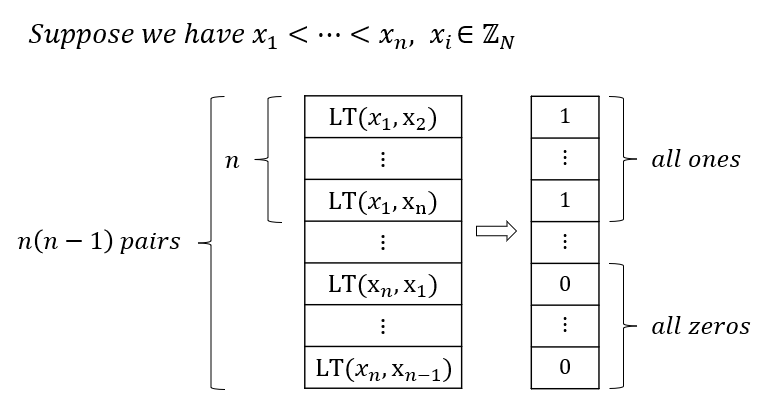
\includegraphics[scale=0.6]{img/fig4.png}%width=\linewidth
	\caption{小数据集上的安全极值协议(SMin(S))}
	\label{smins}
\end{figure}

结果标识为$\{\langle\delta_1\rangle,...,\langle\delta_6\rangle\}$,由云服务器$C_0$和$C_1$秘密共享。然后利用MUL来累乘与$x_i$相关的比较结果,获得$\{\langle m_1 \rangle,\langle m_2 \rangle,\langle m_3\rangle\}$。假设$x_1<x_2<x_3$,与$x_1$相关的比较结果全部为$1$,同时与$x_2$,$x_3$相关的比较结果至少包含一个$0$。因此,对应的累乘结果为$m_1=1, m_2=0, m_3=0$。详细描述如算法\ref{alg_smins}所示,首先用两个数组分别存储待比较的内容,长度为$ n(n-1) $,然后运行安全比较算法获取结果$ \langle t_i \rangle, i \in [1,n(n-1)] $,最后将每一个元素$ x_i $相关的$ n-1 $个比较结果相乘得到最终极值结果$ \langle r_i \rangle, i\in[1,n]$。

\begin{algorithm}[htbp]
	\renewcommand{\algorithmicrequire}{\textbf{输入:}}
	\renewcommand{\algorithmicensure}{\textbf{输出:}}
	\caption{SMin(S) $\rightarrow \{\langle r_1 \rangle,...,\langle r_n\rangle\}$}
	\label{alg_smins}
	\begin{algorithmic}[1]
		\REQUIRE $C_0,C_1$输入$ \{\langle x_1 \rangle,...,\langle x_n\rangle\} $
		\ENSURE $C_0,C_1$获得$\{\langle r_1 \rangle,...,\langle r_n\rangle\}$
		\STATE 构造$ n(n-1) $对比较数据,分别存储在$ l_1 $和$ l_2 $中
		\FOR{$i=1$ to $n$}
		\FOR{$j=1$ to $ n $, $j\neq i$}
		\STATE $ l1[i*(n-1)+j] \leftarrow \langle x_i \rangle $
		\STATE $ l2[i*(n-1)+j] \leftarrow \langle x_j \rangle $
		\ENDFOR
		\ENDFOR
		\STATE 比较大小获取结果$ \langle t \rangle \leftarrow \text{SC}(l1, l2) $
		\FOR{$ i=1 $ to $n$}
		\STATE 将$ \langle x_i\rangle $相关比较结果相乘$ \langle r_i \rangle \leftarrow \text{MUL}(\langle t_{i*(n-1)+1}\rangle,...,\langle t_{i*n} \rangle)$
		\ENDFOR
	\end{algorithmic}
\end{algorithm}

\textbf{针对大型数据集},上述方法增加的比较数据对以平方级剧增,带来大量冗余的通信和计算开销。
因此,这里放弃增加比较数据对的思路,采取树型结构来减少比较轮次,在冒泡排序需要$n-1$轮比较的基础上,将迭代轮次减少为$\log n$。

假设数据集包含$n$个数据,首先比较$n/2$对数据,然后用比较结果与原始数据相乘后相加,以获取一对比较数据中的较小值。以$x$,$y$为例,比较结果为$\delta = LT(x,y) $,较小值的计算方式为$r=\text{MUL}(\delta, y) + \text{MUL}(1-\delta, x)$ 。
经过上述操作数据集的大小由$n$变为$n/2$,保留了所有比较数据对中的较小值。反复进行上述操作,直到集合仅包含一个数据,即极小值,比较过程如图\ref{sminl}所示。
\begin{figure}[htbp]
	\centering
	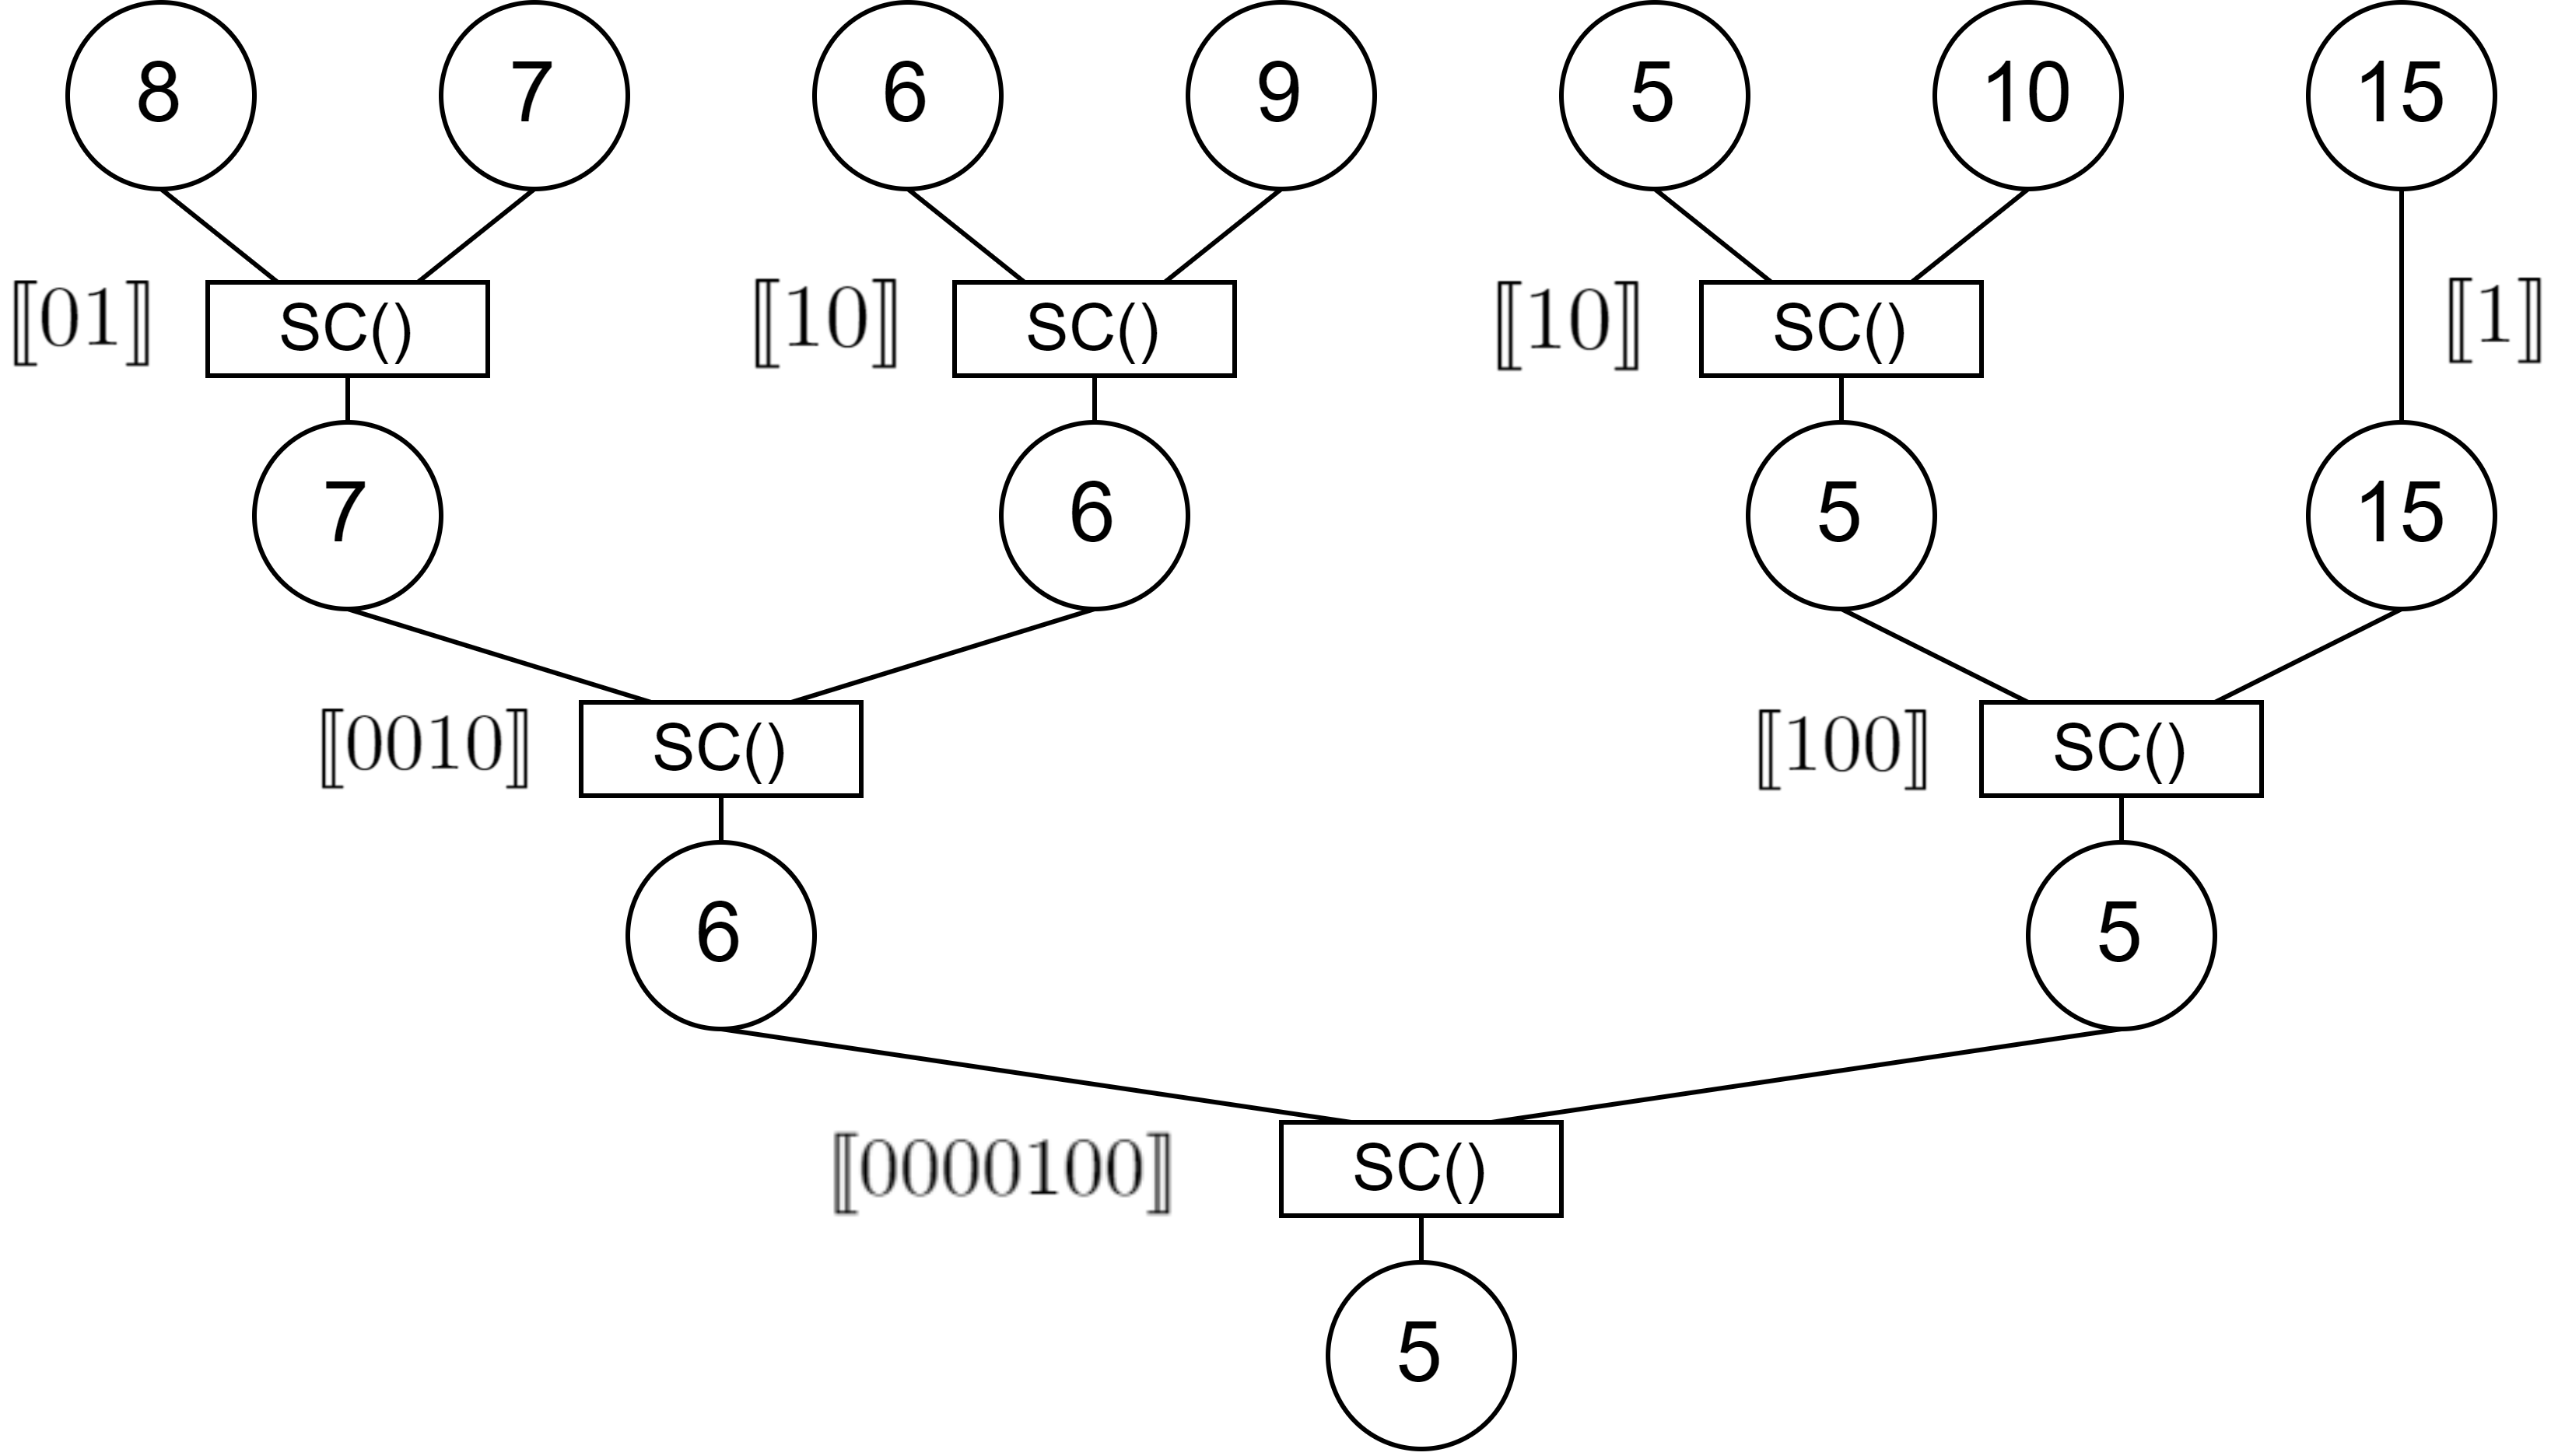
\includegraphics[scale=0.08]{img/fig1.png}%width=\linewidth
	\caption{大数据集上的安全极值协议(SMin(L))}
	\label{sminl}
\end{figure}
\subsection{安全过滤协议}
本节将介绍如何在秘密共享的Kd-tree数据结构上进行聚类,该方案的正确性验证由论文\cite{kanungo2002efficient}给出,明文算法的详细过程在章节\ref{s3-guolvsuanfa}给出。
\begin{algorithm}[htbp]
	\renewcommand{\algorithmicrequire}{\textbf{输入:}}
	\renewcommand{\algorithmicensure}{\textbf{输出:}}
	\caption{SF}
	\label{alg_sf}
	\begin{algorithmic}[1]
		\REQUIRE Kd-tree $\langle tr \rangle$以及初始簇$\{\langle z_j \rangle\}, j\in[k]$
		\ENSURE 新的簇中心$\{\langle z^{\prime}_j\rangle\},j\in[k]$
		\FOR {$i=1$ to $n$}
		\FOR {$j=1$ to $k$}
		\STATE $\langle d_j \rangle \leftarrow$ SED$(\langle z_j \rangle, \langle c_i \rangle)$ %首先计算到每个簇的距离
		\ENDFOR
		\STATE $\{\langle r_1\rangle,...,\langle r_k\rangle\} \leftarrow$ SMin$(\langle d_1 \rangle,...,\langle d_k \rangle)$
		\STATE 计算最近候选簇$\langle z^* \rangle \leftarrow \sum_{p=1}^k$MUL$(\langle r_p \rangle,\langle z_p\rangle)$ %找到最近簇
		\FOR {$j=1$ to $k$} %遍历每个簇
		\STATE $\langle r \rangle \leftarrow$ SC$(\langle u \rangle, 0)$, $\langle \mu \rangle \leftarrow \langle z^{*} \rangle - \langle z_j\rangle$%比较u每个维度和0的大小
		\STATE $\langle v \rangle \leftarrow$ MUL$(\langle r\rangle, \langle c_i \rangle_{min})+ $MUL$(1-\langle r\rangle,\langle c_i\rangle_{max})$
		\STATE $\langle d^{*}\rangle \leftarrow$ SED$(\langle z^{*}, \langle v \rangle)$, $\langle d_j \rangle \leftarrow$ SED$(\langle z_j\rangle,\langle v\rangle)$ %如果prune,z_j就是0
		\STATE $\langle r_j\rangle \leftarrow$ SC$(\langle d^{*}\rangle, \langle d_j\rangle)$
		\ENDFOR
		\STATE $\langle f \rangle \leftarrow$ SC$(\sum_{j=1}^{k}\langle r\rangle_j, 1)$
		\IF{$\langle f \rangle_0 + \langle f \rangle_1 == 1$}
		\STATE $\langle z^{\prime}_j \rangle \leftarrow \langle z^{\prime}_j \rangle +$ MUL$(\langle r_j\rangle, \langle c \rangle),j\in[k]$ %累加
		\ELSE
		\STATE $\langle z_j \rangle \leftarrow$ MUL$(\langle z_j \rangle, \langle r_j\rangle), j\in[k]$
		\STATE 将候选集$\{\langle z_1 \rangle,...,\langle z_k\rangle\}$传递给子节点,并重复上述过程
		\ENDIF
		\ENDFOR
	\end{algorithmic}
\end{algorithm}

自根节点开始,依次遍历所有节点来判断当前节点中包含的所有数据点是否可以被划分到某一个簇中。针对每个节点,维护一个候选簇集合,该集合中所有簇都可能是节点内所有数据的最终所属簇。在迭代中,不断删除不符合条件的候选簇直到仅剩一个候选簇,即节点所属簇。

具体过程如算法\ref{alg_sf}所示。首先,计算Kd-tree中当前节点的中心$ \langle  c_i  \rangle $到每个候选簇中心$ \langle  z_j  \rangle $的距离,然后借助安全极值协议SMin找到距离最近的候选簇并标记为$ \langle z^* \rangle $。
然后,执行一系列子协议来排除不符合候选条件的簇,排除依据为,与候选簇$ \langle z_j\rangle $相比,节点中包含所有数据点在空间上都离$ \langle z^* \rangle $更近,则认为$ \langle z_j \rangle $非候选簇,首先将最近候选簇$ \langle  z^*  \rangle $与其他候选簇$ \langle  z_j  \rangle $按维度相减得到中间结果$ \langle  \mu  \rangle $,然后比较$ \langle  \mu  \rangle $每个维度与0的大小关系得到$ \langle  r  \rangle $,对于$ \langle  \mu  \rangle $中每个值,若小于0,则取当前树节点$ \langle  c_i  \rangle $中该维度数据的最小值,否则取最大值,得到$ \langle  v  \rangle $。分别计算$ \langle  z^*  \rangle $和$ \langle  z_j  \rangle $到$ \langle  v  \rangle $的距离$ \langle  d^*  \rangle $和$ \langle  d_j  \rangle $,比较二者的大小关系。若候选簇$ \langle  z_j  \rangle $被排除,则对应的$ \langle  r_j  \rangle $的结果为0,否则为1。更加详细的规则解释在论文\cite{kanungo2002efficient}中给出。
在此之后,累加结果并执行安全比较协议来判断候选簇集合是否仅剩一个簇。
如果是,则将节点中所有数据划分到新簇$ \langle  z^{\prime}_j  \rangle $中,并停止向下迭代,否则继续对子节点重复上述操作。若聚类过程即将收敛,那么能够快速排除其他簇进行划分,子节点可以不用进行冗余的距离计算和比较,节省大量计算资源。
然而上述方案泄露了一比特数据来判断是否终止子节点迭代,这样少量的数据仅仅轻微泄露了迭代过程的信息,但是带来了效率的巨大提升。论文\cite{bozdemir2021privacy,boldyreva2021privacy}中采取了类似的方法作为一个交换来获取性能提升。

值得一提的是,不同节点之间包含的数据不相交,并且划分的过程和结果不会相互影响,因此可以引入并行处理来加速不同节点之间处理和计算,进一步提升安全过滤算法的效率。

\section{基于Kd-tree的隐私保护K-means方案}
\label{s3-ppokc}
本节主要介绍基于Kd-tree的隐私保护K-means方案(PPOKC)的具体细节。假设数据在双云服务器$C_0$和$C_1$上加性秘密共享,并且二者不可以合谋。云服务器在密文基础上进行系列安全协议获取聚类结果,整个过程可以被划分为两个阶段:
\begin{compactitem}
	\item \textbf{初始化}:首先,用户基于拥有的明文数据构建Kd-tree。然后将数据秘密共享为两份,并分别发送给云服务器$C_0$和$C_1$。此外,原始数据也会在被划分后发送给云服务器以支持其他计算。此后用户不再参与聚类过程。
	\item \textbf{聚类}:对Kd-tree中节点执行过滤操作,根节点的候选簇集合包含所有初始簇。针对树中的节点,执行过滤操作,直到所有数据都被划分到对应的簇。在每轮迭代结束,更新簇中心并且将新簇与旧簇相比较来判断是否满足聚类收敛条件。
\end{compactitem}

\subsection{算法详述}
PPOKC方案的细节在算法\ref{alg_ppokc}中给出,虽然这里提供了一种判断是否停止迭代的方法,在稍后的实验中会采取固定迭代次数的方式来测试性能。
不同的数据集迭代收敛所需的轮次通常不同,目前许多相关隐私保护聚类研究采取的迭代终止策略通常存在安全问题,即泄露数据集迭代收敛所需轮次或者泄露了一定的数据。同时,K-means聚类算法在迭代足够多轮次后一定会收敛\cite{mohassel2019practical}。


\begin{algorithm}[htbp]
	\renewcommand{\algorithmicrequire}{\textbf{输入:}}
	\renewcommand{\algorithmicensure}{\textbf{输出:}}
	\caption{隐私保护外包聚类算法}
	\label{alg_ppokc}
	\begin{algorithmic}[1]
		\REQUIRE 明文数据$x_{ij},i\in[n],j\in[m]$
		\ENSURE 秘密共享的簇中心$\langle z'_j \rangle,j\in[k]$
		\STATE \textbf{初始化(用户)}
		\STATE 在明文基础上构造Kd-tree
		\STATE 加性秘密共享数据$x_{ij}$以及Kd-tree,随机选择初始簇中心$z_j,j\in[k]$,上述内容分别发送给$C_0$和$C_1$
		\STATE \textbf{聚类($C_0,C_1$)}
		\STATE $\{\langle z^{\prime}_1 \rangle,...,\langle z^{\prime}_k\} \leftarrow$ SF$(\langle z_1\rangle,...,\langle z_k\rangle)$
		\STATE $\langle r \rangle \leftarrow \sum_{i=1}^{n}\sum_{j=1}^{m}$SC$(\langle z_{ij}\rangle-\langle z_{ij}^{\prime}\rangle, 1)$
		\IF{$\langle r \rangle_0 + \langle r\rangle_1 == 1$}
		\STATE 终止迭代,返回结果给用户
		\ELSE
		\STATE $\{\langle z_1 \rangle,...,\langle z_k \rangle \} \leftarrow \{\langle z^{\prime}_1 \rangle,...,\langle z^{\prime}_k\rangle\}$
		\STATE 回到步骤5
		\ENDIF
	\end{algorithmic}
\end{algorithm}

\subsection{讨论}
\label{taolun}
最近,论文\cite{wu2020secure}提出了一种双云环境下基于密文打包技术的高效隐私保护K-means聚类方案。然而,虽然方案非常高效,但是存在一些安全性问题。在论文\cite{wu2020secure}的S3ED算法中11行,可以看到$D s t_{a j} \leftarrow Dst_{a j} * r_1^a+r_1^a$, for $j \in[k]$,意味着距离矩阵中行$ a $中所有值均被添加相同的噪声。根据论文\cite{liu2019toward}章节7.3的分析,上述方式无法保护数据的分布信息。在本方案中,不同的距离均为秘密共享值,在进行安全比较时,添加了互异的随机噪声,因此不会泄露原始数据任何相关信息。


\section{安全性分析}
\label{s3-lilun}
本节中,根据论文\cite{goldreich2004encryption}中的标准模拟理论,假设双云服务器$ C_0$和$ C_1$为潜在的攻击者,并提供对于安全欧式距离、安全比较协议、安全极值协议、以及安全过滤协议的书面安全性证明。然后,根据组合理论,证明PPOKC方案在半诚实模型下是安全的。 为了论证方案的安全性,首先介绍半诚实模型下的安全性定义\cite{bogdanov2008sharemind}:
%https://www.cs.jhu.edu/~abhishek/classes/CS600-642-442-Fall2018/L12.pdf 偷的定义
\begin{definition}
	参与方$ A $和$ B $在半诚实模型下计算函数$ f $,若存在一对非均匀的概率多项式模拟器$ S_A,S_B $,以使得对于每一个安全参数$ n $和所有输入$ x,y\in\{0,1\}^n $,都有以下内容成立:
	\begin{equation}
		\begin{aligned}
			 & \left\{\mathcal{S}_A(x, f(x, y)), f(x, y)\right\} \approx\left\{e \leftarrow[A(x) \leftrightarrow B(y)]: \operatorname{View}_A(e), \operatorname{Out}_B(e)\right\} \\
			 & \left\{\mathcal{S}_B(y, f(x, y)), f(x, y)\right\} \approx\left\{e \leftarrow[A(x) \leftrightarrow B(y)]: \operatorname{View}_B(e), \operatorname{Out}_A(e)\right\}
		\end{aligned}
	\end{equation}
\end{definition}

此外,证明中需要用到如下引理:

\begin{lemma}
	\label{s3-lemma1}
	如果一个随机元素$ c $在$ \mathbb{Z}_N $上是随机分布的,且与$ \mathbb{Z}_N $中的元素$ x $无关,则$ c\pm x$在$ \mathbb{Z}_N $也是均匀随机分布的,与$ x $的值无关。
\end{lemma}

接下来开始证明相关协议的安全性:

\begin{theorem}
	安全欧式距离计算协议在半诚实模型下是安全的。
\end{theorem}
\begin{proof}
	安全欧式距离计算协议中,大部分计算由云服务器$ C_0 $和$ C_1 $分别在本地进行,没有泄露可能性。交互操作仅在乘法部分,该方法的安全性证明已经由论文\cite{beaver1992efficient}给出。因此,根据组合理论,本协议的安全性得证。
\end{proof}

\begin{theorem}
	安全比较协议在半诚实模型下是安全的
\end{theorem}
\begin{proof}
	该算法是基于文献\cite{rathee2020cryptflow2}中的百万富翁协议,对输入和输出进行改造。$ C_0 $用不同的随机数打乱数据,然后发送给$ C_1 $,这种方式根据引理\ref{s3-lemma1}是安全的。输出部分,由布尔秘密共享值转换为加性秘密共享值的安全证明依赖于乘法的安全性。因此,证明安全比较协议是安全的。
\end{proof}
\begin{theorem}
	安全极值协议在半诚实模型下是安全的。
\end{theorem}
\begin{proof}
	小数据集上的安全极值协议是安全比较协议的变形,唯一的区别是在协议最后添加了一些乘法操作,因此安全性可以由安全比较协议推导出。对于大数据集上的安全极值协议,令云服务器$ C_1 $的执行镜像为$\Pi_A(S C)=\left\{x_i^A, r_i^A, \alpha_i^A\right\}$,其中$ x_i^A $为输入值,$ r_i^A $为中间值以及$ \alpha_i^A $为比较结果,其中$ i,j\in[n] $。上述所有值均为秘密共享值。假设$ C_1 $的模拟镜像表示为$\Pi_A^S(S C)=\left\{x_i^{\prime}, r_i^{\prime}, \alpha_i^{\prime}\right\}$,模拟镜像中所有值都是$ \mathbb{Z}_N $上的随机值。由于秘密共享均为$ \mathbb{Z} $上的随机值,因此$ \left\{x_i^A, r_i^A, \alpha_i^A\right\} $与$ \left\{x_i^{\prime}, r_i^{\prime}, \alpha_i^{\prime}\right\} $计算上不可区分。根据上述分析,可以认为$ \Pi_A(SC) $与$ \Pi_A^S(SC) $计算上不可区分。$ C_1 $和$ C_0 $执行的相同的工作,所以在这里省略重复分析。
\end{proof}
\begin{theorem}
	本文所述的隐私保护外包K-means聚类方案在半诚实模型下是安全的。
\end{theorem}
\begin{proof}
	从\ref{alg_ppokc}中可以看出,所述PPOKC方案是由上述安全协议组成的。在前面已经给出了基础安全协议的安全性证明,根据组合原理\cite{goldreich2004encryption},可以认为PPOKC方案在半诚实模型下是安全的。此外,由于云平台$ C_0 $和$ C_1 $是不能合谋的,因此它们也无法获知每个数据具体划分到哪个簇中,所以数据的访问模式也得到了保护。由于Kd-tree的数据结构特点,决定了每个节点中包含数据的个数已知,但是具体包含哪些数据是未知的,因此云平台无法跟踪数据与树节点的关系。
\end{proof}
\section{系统评估与性能分析}
\label{s3-shiyan}
前述内容详细的描述方案中涉及协议的具体涉及以及相关知识,本节在依据方案实现系统的基础上详细进行理论分析和实验评估,在多个人工合成的数据集上进行实验以观察系统的实用性和可扩展性。同时,也在现实数据集上进行了充分的实验,以和目前最先进的隐私保护K-means聚类方案\cite{wu2020secure,mohassel2019practical}进行实验对比。
\subsection{理论分析}
本节中,主要从理论层面分析方案的计算和通信开销。安全欧式距离仅包含简单的秘密共享加法和乘法运算,因此不纳入分析。安全比较算法主要基于论文\cite{rathee2020cryptflow2}中的百万富翁协议,详细的效率分析已经在论文中给出,这里不再赘述。因此主要分析安全极值协议以及安全过滤协议。值得注意的是,乘法所需三元组的计算是离线进行的,因此这里生成乘法三元组的过程不纳入计算与通信开销分析。
\subsubsection{计算开销}
考虑到上述两个协议,主要由安全比较和秘密共享乘法加法组成,乘法与加法相对安全比较协议来说计算开销可以忽略不计,因此在以下的论述中,以安全比较协议的运行次数为基准给出分析结果,如表\ref{s3-table-compucost}所示:
\begin{table}[htbp]
	\centering
	\renewcommand{\arraystretch}{1.3}
	\caption{计算开销理论分析}
	\label{s3-table-compucost}
	\scalebox{1.0}{
		\begin{tabular}{c|c|c|c}% 通过添加 | 来表示是否需要绘制竖线c|
			\hline  % 在表格最上方绘制横线
			协议         & 安全极值协议(大数据集) & 安全极值协议(小数据集) & 安全过滤协议 \\%&SKD
			\hline % 在表格最下方绘制横线
			安全比较协议 & $\log n$               & $1$                    & $2kn$        \\%$n^2\log n$
			\hline
		\end{tabular}
	}
\end{table}

借助安全比较协议,可以运行一轮协议比较多对数据,效率非常高。然而,随着比较数据的增加,计算开销也随之剧增。虽然小数据集上的安全极值协议只需要运行一次安全比较协议,但是当数据量变得很大时,协议运行非常耗时。因此设计了另一种能够减少比较数据量略微增加比较次数的协议。

\subsubsection{通信开销}
假设数据集大小为$ n $,数据为$ l$比特,这里仅分析乘法的通信开销,因为安全比较协议的通信开销分析比较复杂,并且在论文\cite{rathee2020cryptflow2}中已经给出。在安全比较协议,以及小数据集上的安全极值协议,通信开销分别为$ 3nl $,$ 7n(n-1)l $比特。对于大数据集上的安全极值协议,开销最多不超过$ nl\log n $比特。因为安全过滤协议的开销分析非常复杂,这里仅给出近似值$ O(n^2\log n)l $比特。
\subsection{实验分析}
本节通过实验评估本文所述方案的性能,我们基于c++编程语言和论文\cite{rathee2020cryptflow2}中的函数库实现了整个系统,并对用户与云平台以及云平台之间的交互进行了仿真模拟。我们主要关注系统在不同的数据集上的计算和通信开销,以及与论文\cite{wu2020secure,mohassel2019practical,jaschke2019unsupervised}在相同数据集上的实验表现进行对比。

为了与前沿研究论文\cite{wu2020secure,mohassel2019practical}的实验进行直观的对比,我们选择完全相同的实验机器,配置为Inter Core i7-7700HQ 2.80 GHz CPU和16 GB RAM。然而,上述机器内存有限,为了进一步考察方案的可扩展性,我们选择在配置为Intel Core i9-10980XE 3.00GHz CPU 和 64GB RAM的机器上对人工合成的数据集进行系列实验,考察簇个数$k$、数据量$n$和数据维度$m$对于系统性能的影响。
\subsubsection{数据集}
\begin{table}[htbp]
	\centering
	\renewcommand{\arraystretch}{1.3}
	\caption{数据集详细信息}
	\label{s3-dataset}
	\scalebox{1.0}{
		\begin{tabular}{c|c|c|c}% 通过添加     | 来表示是否需要绘制竖线
			\hline  % 在表格最上方绘制横线
			数据集名称 & 数据集大小 $n$    & 簇个数 $k$ & 维度 $d$   \\
			\hline % 在表格最下方绘制横线
			Lsun       & $400$             & $3$        & $2$        \\
			\hline  %在第一行和第二行之间绘制横线
			KEGG       & $8192$            & $3$        & $5$        \\
			\hline
			Synthetic  & $\{10000,60000\}$ & $\{3,15\}$ & $\{2,20\}$ \\
			\hline
		\end{tabular}
	}
\end{table}
为了能够进行全面的对比,这里使用了表格\ref{s3-dataset}所示数据集,其中每一个都在之前的研究工作中出现过:
\begin{compactitem}
	\item \textbf{KEGG:}是一个集成的数据库,主要包含15个不同的数据库资源,包含的内容主要是分子系统的计算机表示,从基因信息到化学信息等。本方案选择的KEGG Metabolic Reaction Network(Undirected),是收录于UCI KDD条目的现实世界数据集\cite{naeem2011kegg}。本文从中提取8192条数据,5个维度($ n=8192,m=5 $),令簇个数$ k=3 $进行实验,以和论文\cite{wu2020secure}的实验设置保持一致。
	\item \textbf{Lsun:}数据集是来自论文\cite{franti2018k}的一个人造二维数据集,该数据集常用于聚类研究以进行对比分析和展示。其中包含400个数据,3个簇。将用于与论文\cite{jaschke2019unsupervised}的比较。
	\item \textbf{人工合成数据集:}本文构造了数据量为$ n $,维度为$ m $的人造数据集,随机值为整数,均匀分布在$ [0,1000] $内。簇的个数在3到15之间以方便进行实验。
\end{compactitem}

\subsubsection{现实数据集上的实验}
\textbf{与论文\cite{wu2020secure}方案对比}:为了进行最直接的比较,这里使用相同的数据集和一致的实验机器运行本系统。实验数据如表格\ref{s3-ta-duibi}所示,其中给出了PPCOM\cite{rong2017privacy}、SEOKC\cite{wu2020secure}以及本方案PPOKC进行一轮迭代的通信和计算开销。

\begin{table}[htbp]
	\centering
	\renewcommand{\arraystretch}{1.3} % 调整行高度
	\caption{通信与计算开销对比($n=8192,m=5,k=3$)}
	\label{s3-ta-duibi}
	\scalebox{1.0}{ % 缩放表格
		\begin{tabular}{c|c|c|c}% 通过添加 | 来表示是否需要绘制竖线
			\hline  % 在表格最上方绘制横线
			实验表现 & PPCOM   & SEOKC  & PPOKC \\
			\hline  %在第一行和第二行之间绘制横线
			计算开销 & 401 min & 17 s   & 20 s  \\
			\hline % 在表格最下方绘制横线
			通信开销 & 1430 MB & 148 MB & 405MB \\
			\hline
		\end{tabular}
	}
\end{table}
从计算耗时角度来看,PPCOM方案和SEOKC方案迭代一轮分别需要401分钟和17s,而本文的PPOKC方案则需要20s,对比来看,比PPCOM方案要快1203倍,比SEOKC方案慢3s。从通信开销角度来看,PPCOM需要1430MB而SEOKC需要148MB,本方案则需405MB。

综合来看,本文的方案的表现远远超过PPCOM,接近目前最高效的SEOKC方案。值得一提的是,从章节\ref{taolun}可以看到,SEOKC方案虽然高效但是存在不容忽视的安全性问题,采取的随机噪声方法会暴露数据分布。而PPOKC方案则更加安全,不会泄露相关信息,因此性能上略微逊色是可以接受的。

\textbf{与论文\cite{jaschke2019unsupervised}的比较}:为了进行公平的比较,这里在Lsun数据集上进行实验。对比论文的机器为Inter i7-3770 3.4GHz 20GB RAM,本文所用前述实验机器要慢1.3倍。

论文\cite{jaschke2019unsupervised}提供了3种不同的隐私保护K-means聚类方案,分别是精确的、稳定的以及近似的方案。上述方案进行15轮迭代分别用时为545.91天、48.9小时、15.47小时。在本文的系统中,完成相同的迭代轮次总共需要20.94秒,用时远远少于前述三种方案。

此外,实验设置相同的初始簇中心初始化,在Lsun数据集上分别运行明文K-means方案以及本文提出的PPOKC方案,分类结果如图\ref{f4}和图\ref{f5}所示。本方案所有安全协议的正确性均以论文\cite{kanungo2002efficient}中提出的基于Kd-tree的改进K-means方案为支撑。因此,最终聚类结果和明文方案完全一致。

\begin{figure}[htbp] %[htbp]
	%	\captionsetup{font=scriptsize}
	\begin{minipage}[t]{0.5\linewidth}
		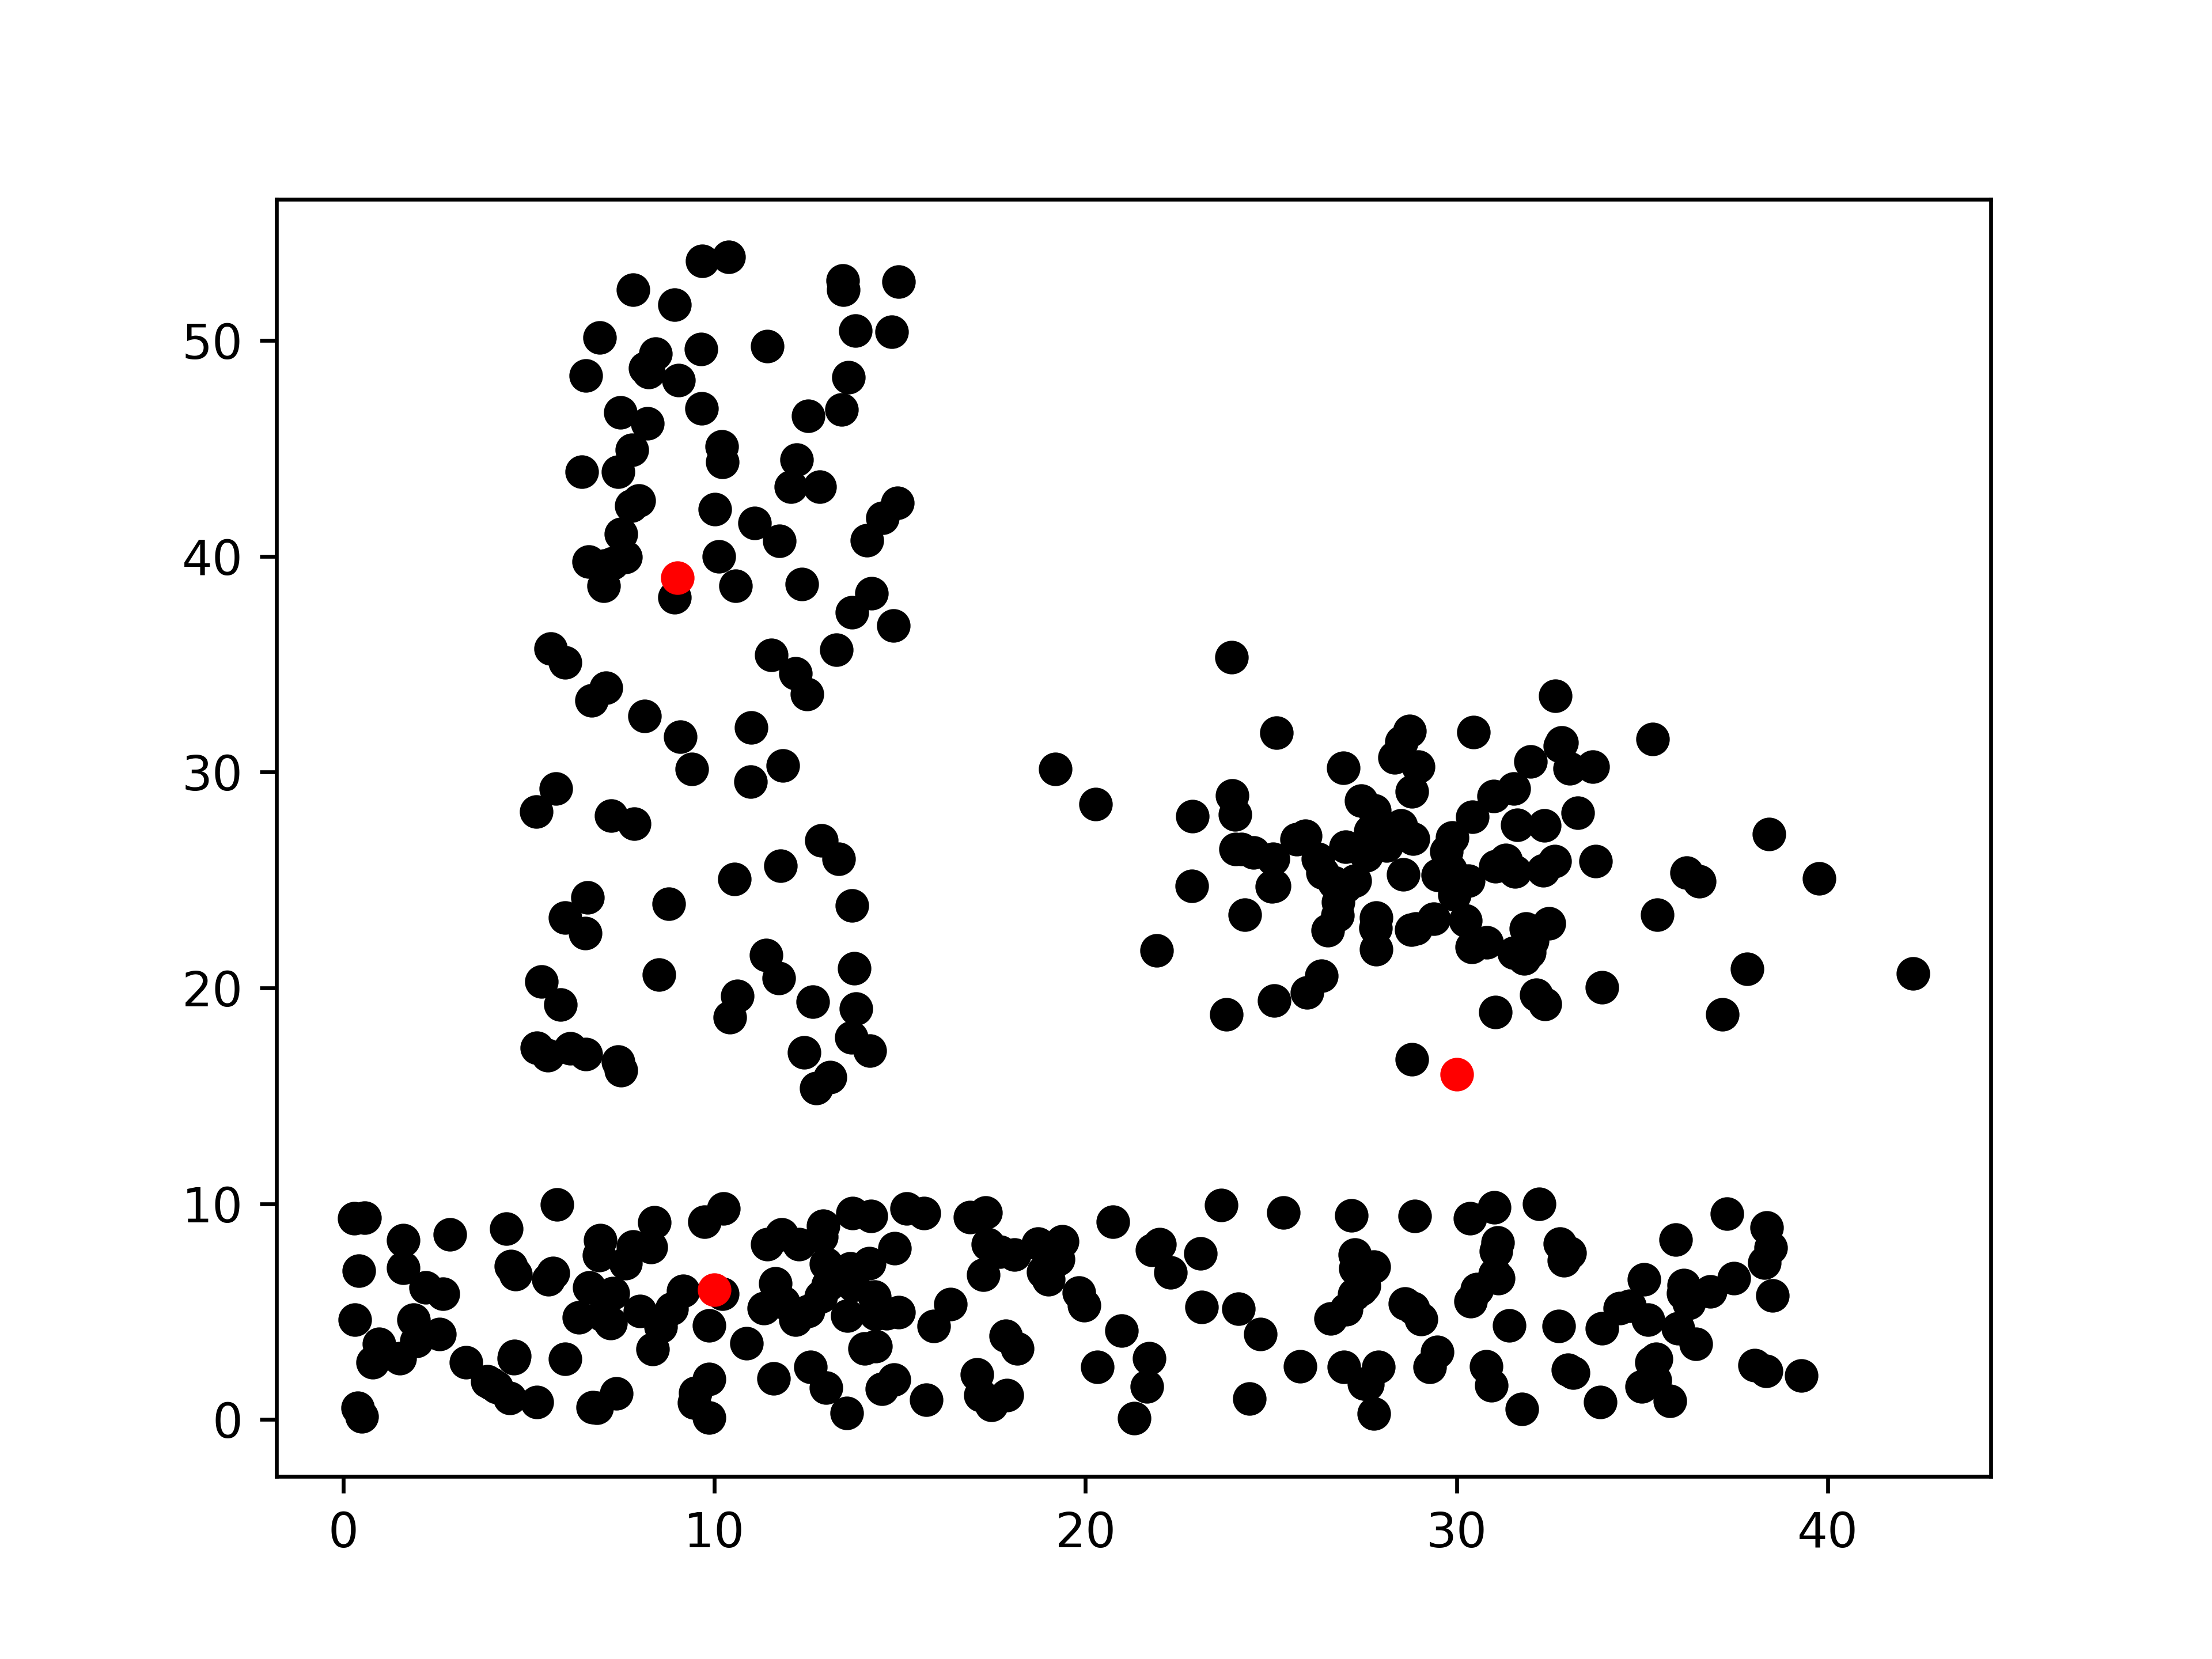
\includegraphics[width=\linewidth]{img/lsun_ptxt.png}
		\caption{明文K-means聚类结果}
		\label{f4}
	\end{minipage}%
	\hfill%
	\begin{minipage}[t]{0.5\linewidth}
		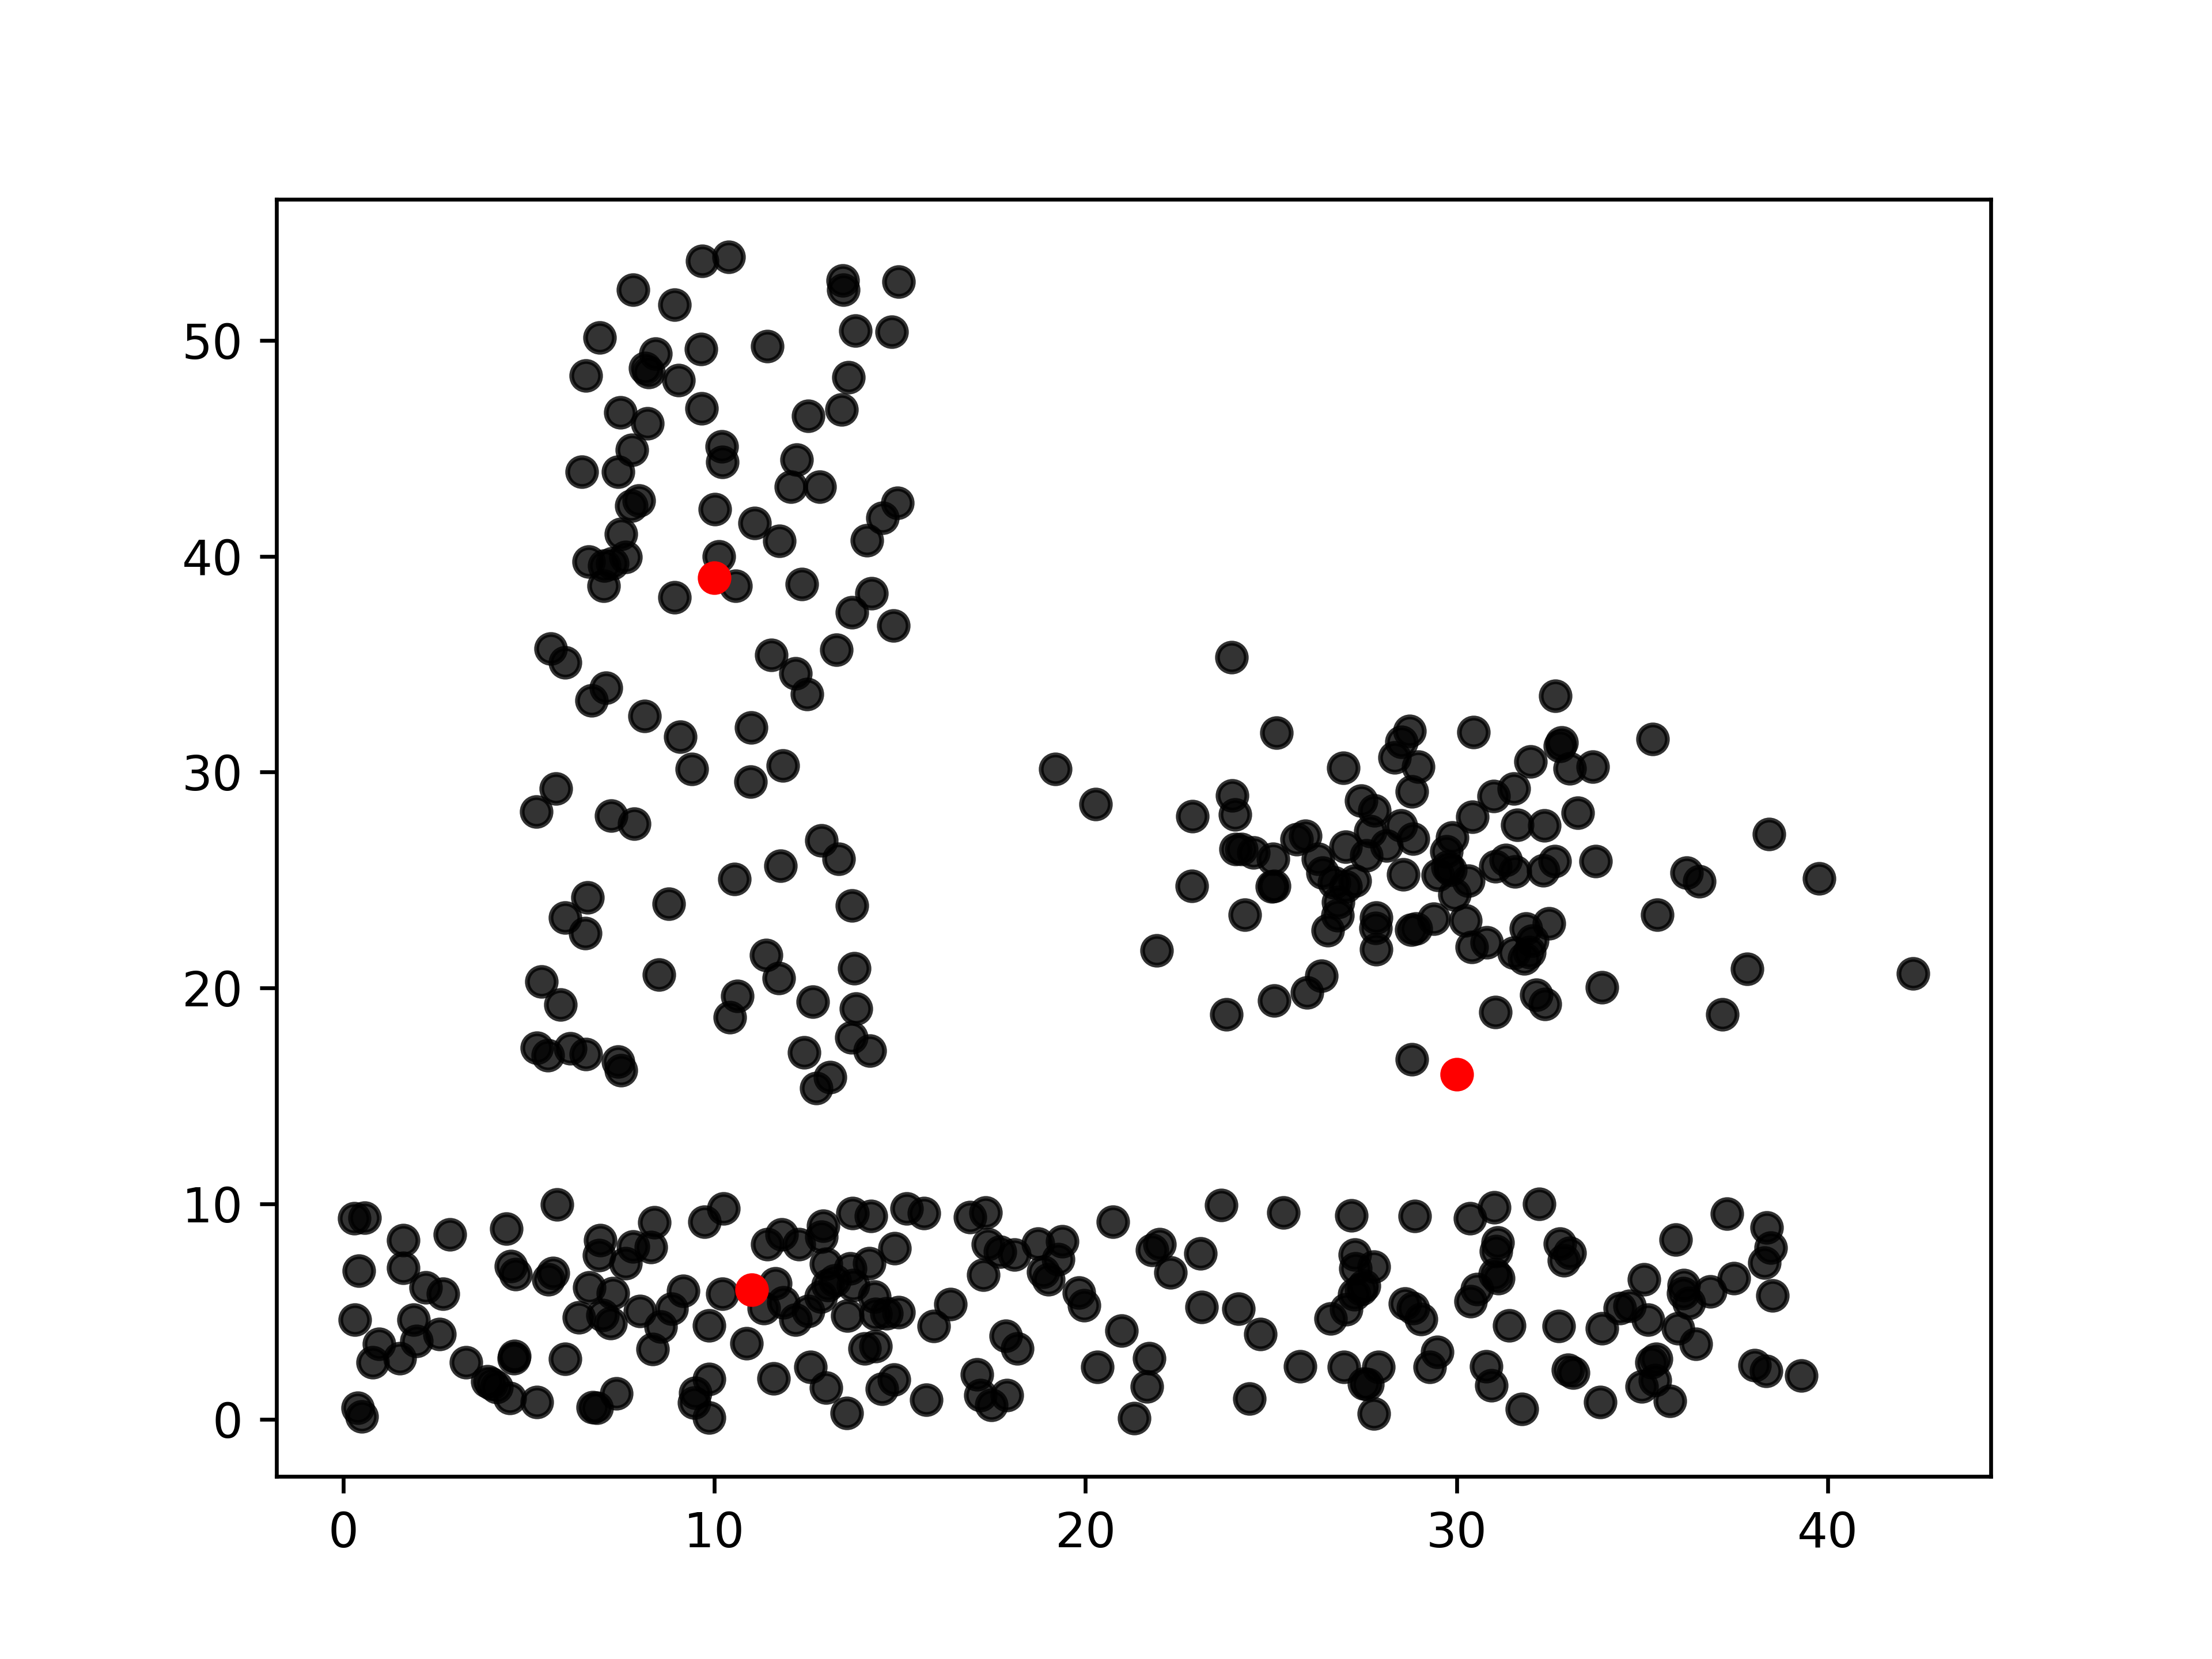
\includegraphics[width=\linewidth]{img/lsun_ctxt.png}
		\caption{隐私保护K-means方案聚类结果}
		\label{f5}
	\end{minipage}
\end{figure}
\subsubsection{人造数据集上的实验}
%todo 图画错了家人们
本节,在数据量跨度为$ n\in[10000,60000] $的人造数据集上进行系列对比实验。在生成数据时控制簇的个数在3-15之间,彼此之间没有重叠的部分。同时,聚类终止条件选择达到指定迭代次数即停止聚类比较结果。该选择主要原因如下:不同数据集收敛所需迭代次数不固定,受初始簇中心的影响较大,若按照算法中所给出的判断是否收敛来停止迭代,会导致时间分析不准确。

这里考虑三个影响聚类的参数,分别是数据集大小$ n $、数据的维度$ m $以及簇的个数$ k $。为了准确的分析参数对于方案的性能影响,本文的策略是固定一个参数,然后变化另外两个参数的值来运行系统。实验运行的计算和通信开销如图\ref{f6}和图\ref{f7}所示。

\begin{figure}[htbp] %[htbp]
	\begin{minipage}[t]{0.5\linewidth}
		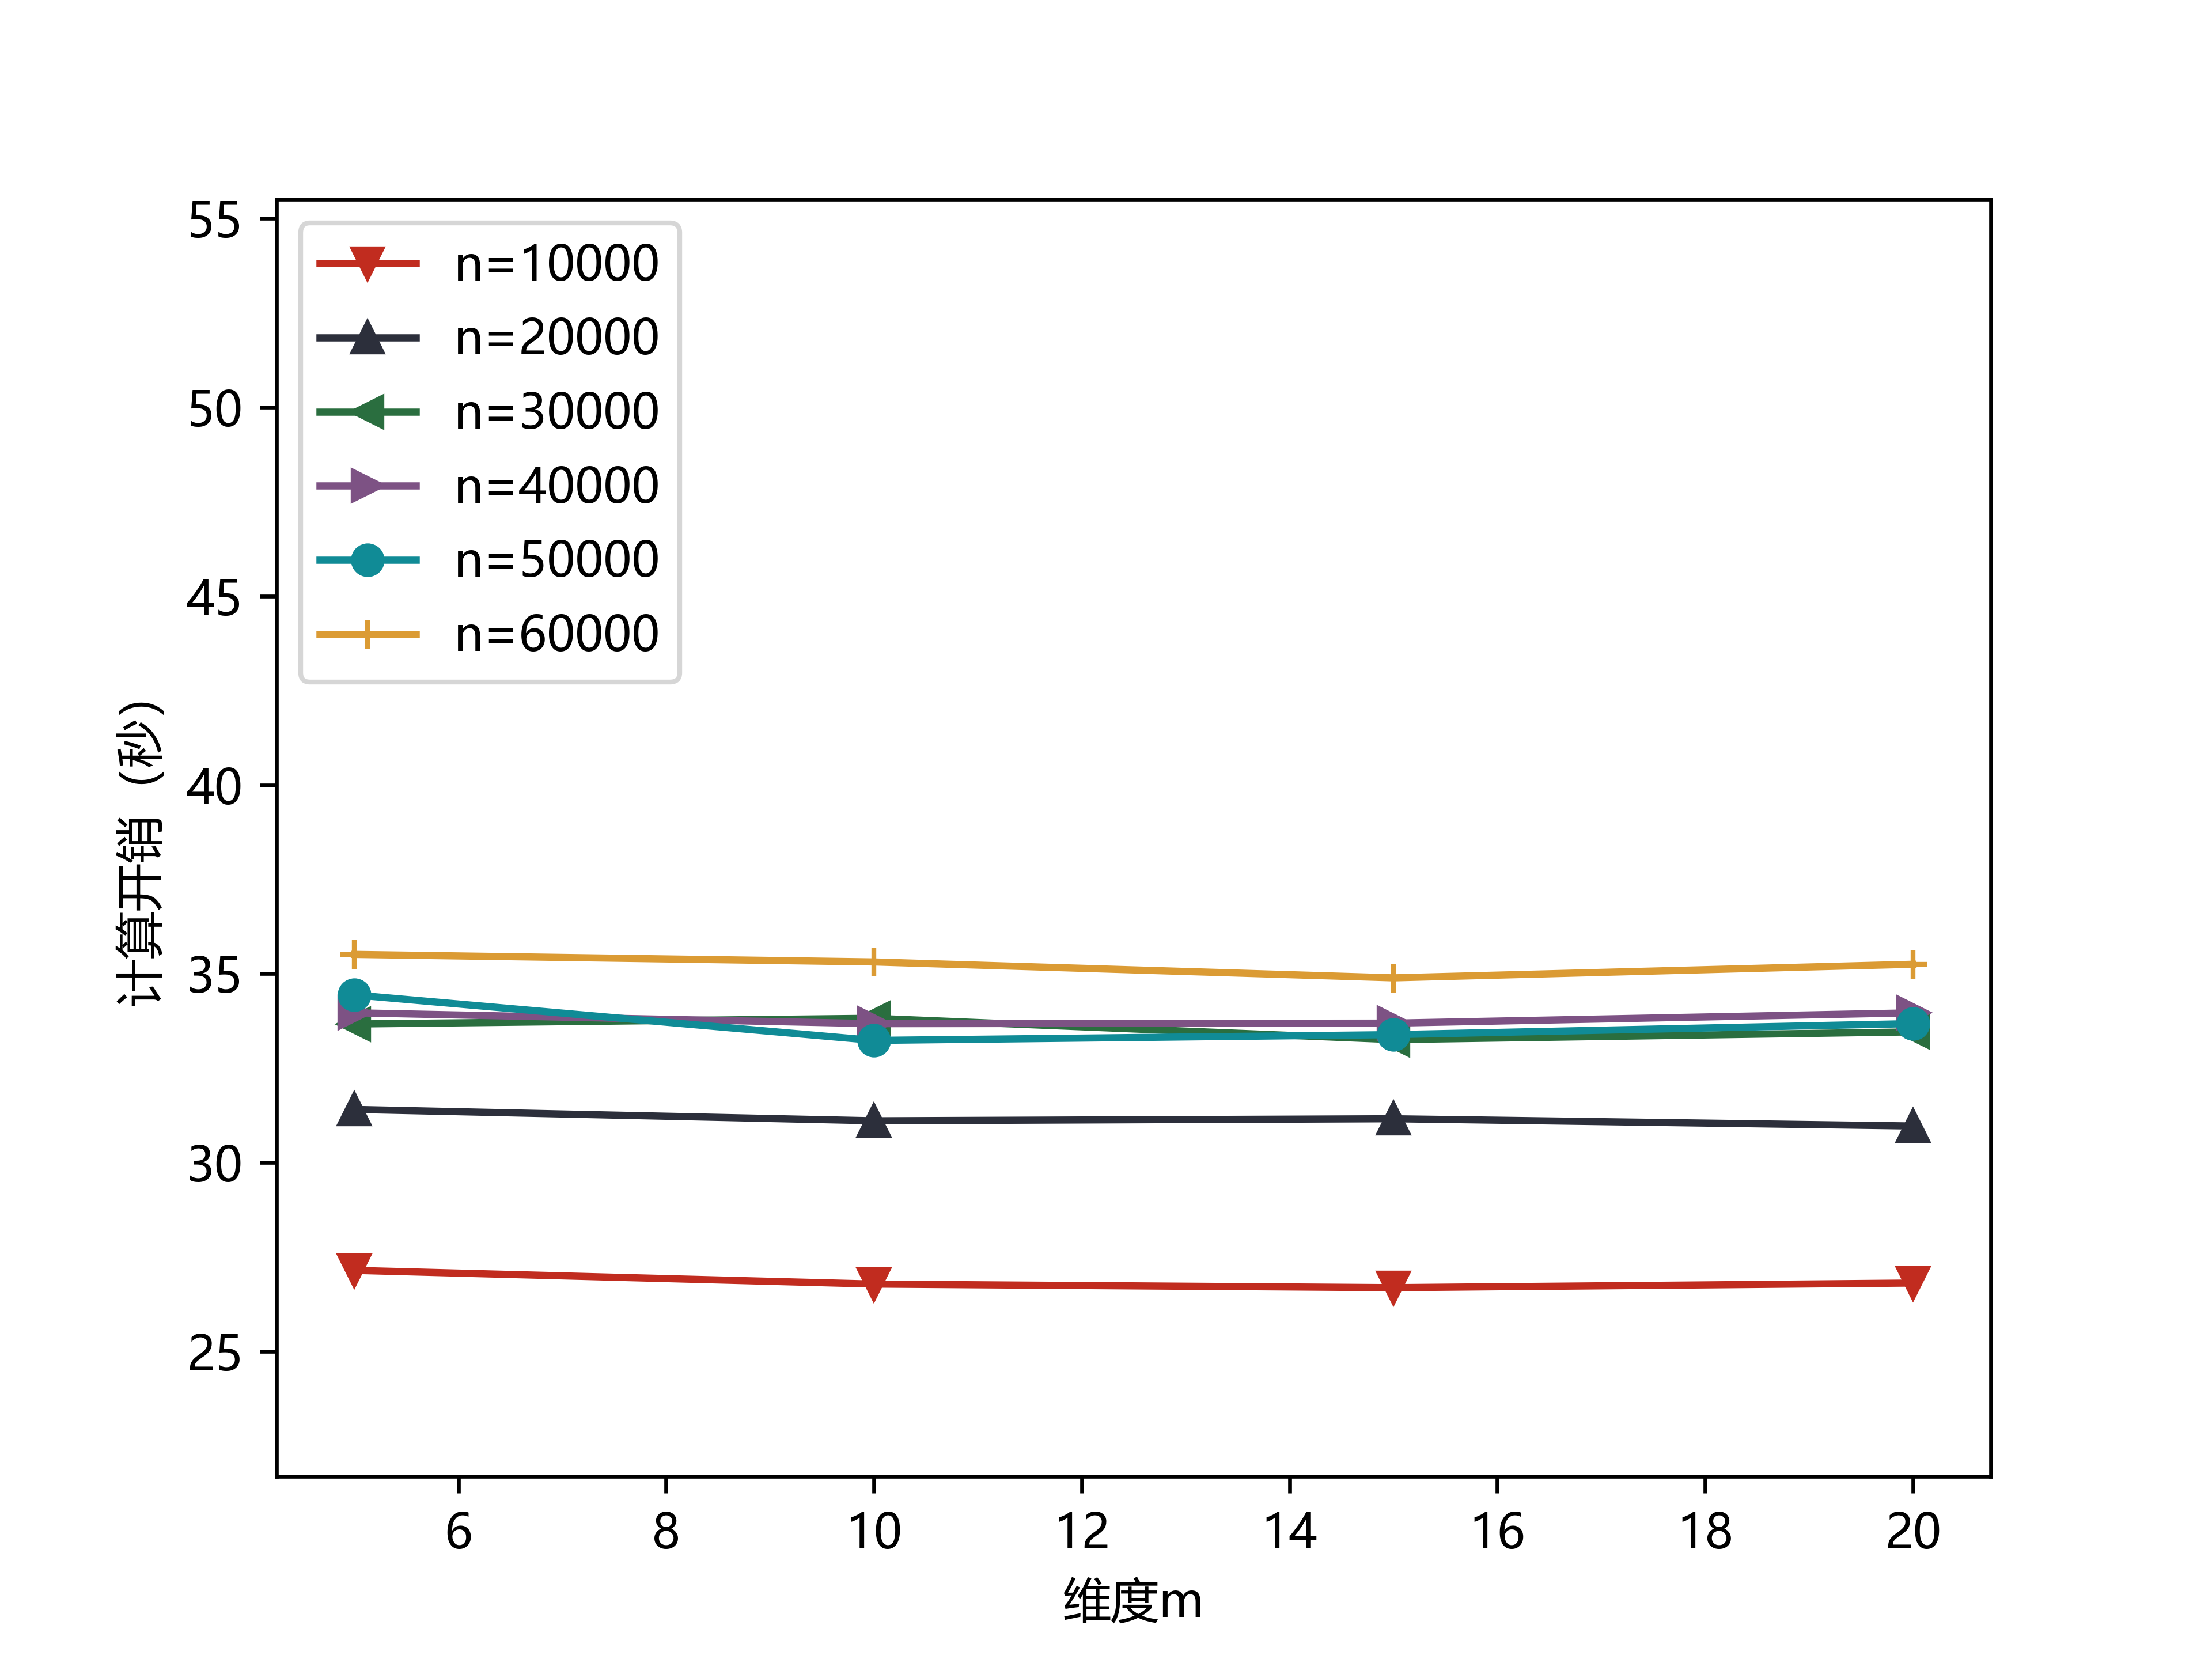
\includegraphics[width=\linewidth]{img/newm_time.png}
		
	\end{minipage}%
	\hfill%
	\begin{minipage}[t]{0.5\linewidth}
		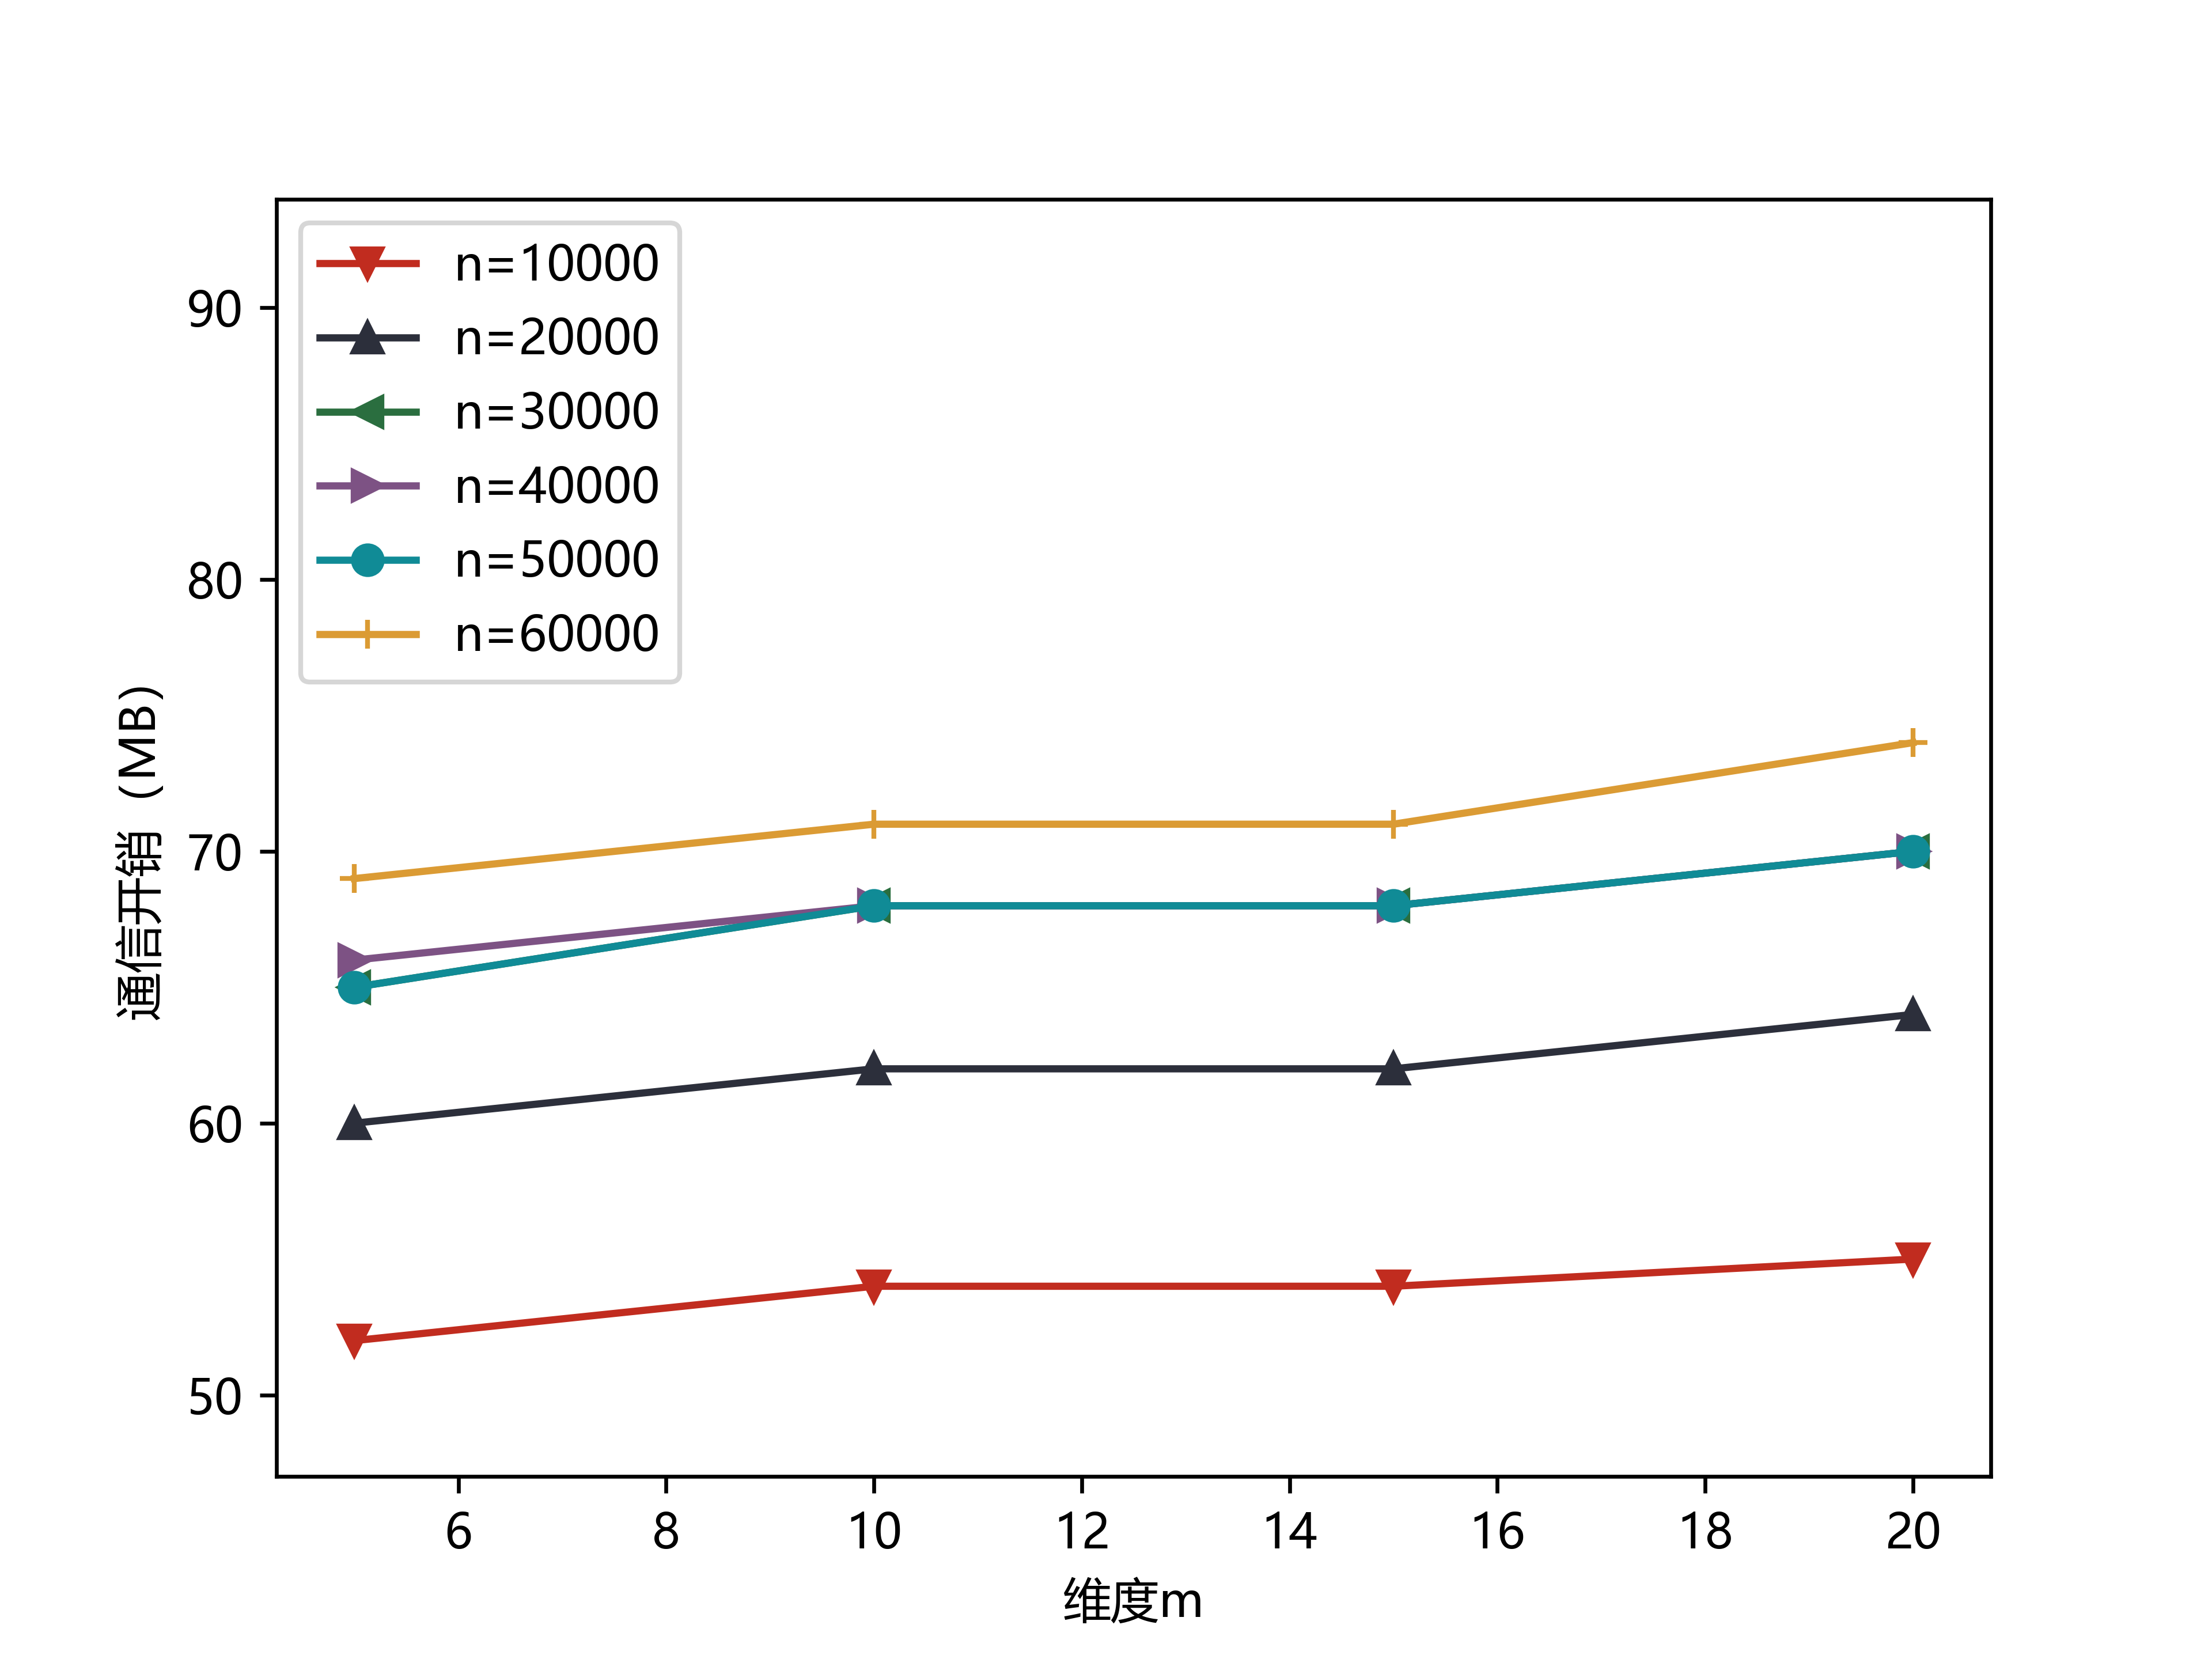
\includegraphics[width=\linewidth]{img/newm_comm.png}
		
	\end{minipage}
	\caption{维度$ m $对方案开销的影响}
	\label{f6}
\end{figure}

对于图\ref{f6},这里固定$k=3, T=20$,变化维度$ m $的大小来观察计算和通信开销的变化。
首先从曲线的变化可以看到计算开销和通信开销的变化趋势相似,其次二者均随着数据量$ n $的增加而增加,但是从跨度来看,随着$ n $的变化,计算开销和通信开销的跨度均较小,原因在于人工合成的数据集,数据分布比较规范,同时实验中令初始簇中心选择在每个生成的簇内,因此算法会快速收敛,冗余计算大大减少。
维度$ m $对两种开销的影响几乎可以忽略不计。具体原因在于,维度的变化只会对密文计算中的加法和乘法次数产生影响,不会影响安全比较协议的运行次数,而后者才是隐私保护聚类方案的瓶颈,此外,乘法操作的次数还可以通过引入并行操作进行优化,进一步减少开销。

\begin{figure}[htbp]
	%	\captionsetup{font=scriptsize}
	\begin{minipage}[t]{0.5\linewidth}
		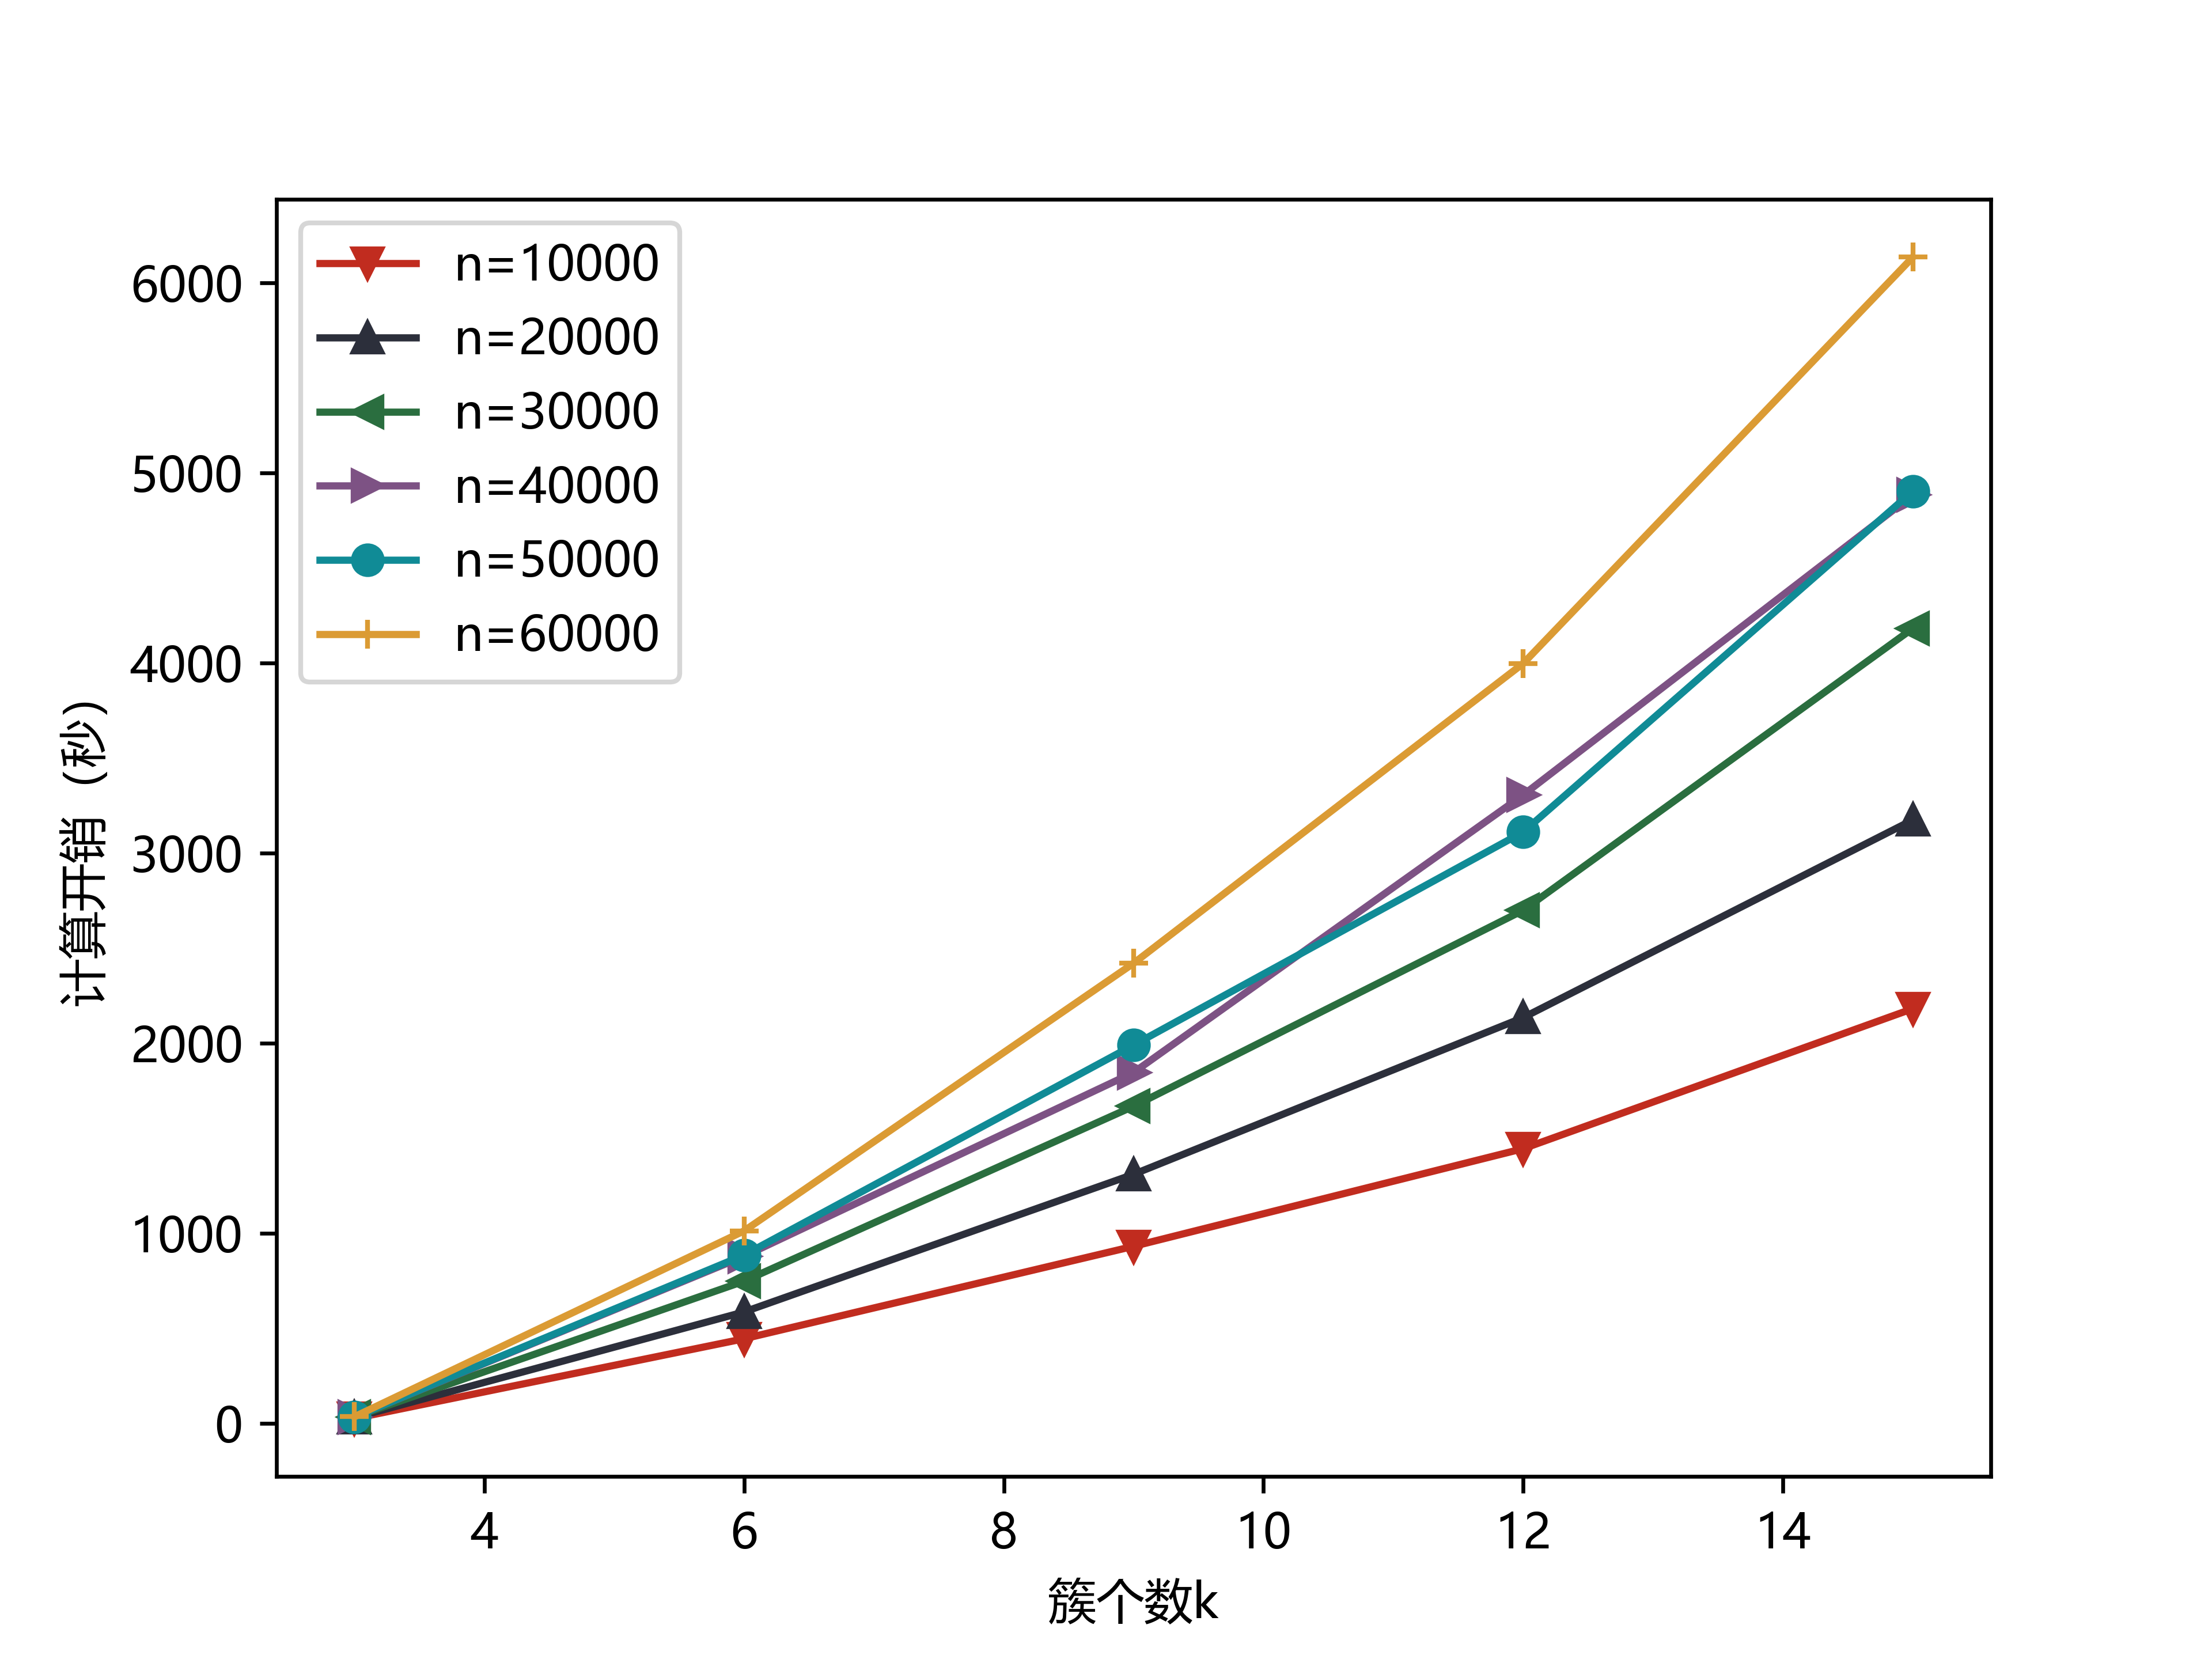
\includegraphics[width=\linewidth]{img/newk_time.png}
		
	\end{minipage}%
	\hfill%
	\begin{minipage}[t]{0.5\linewidth}
		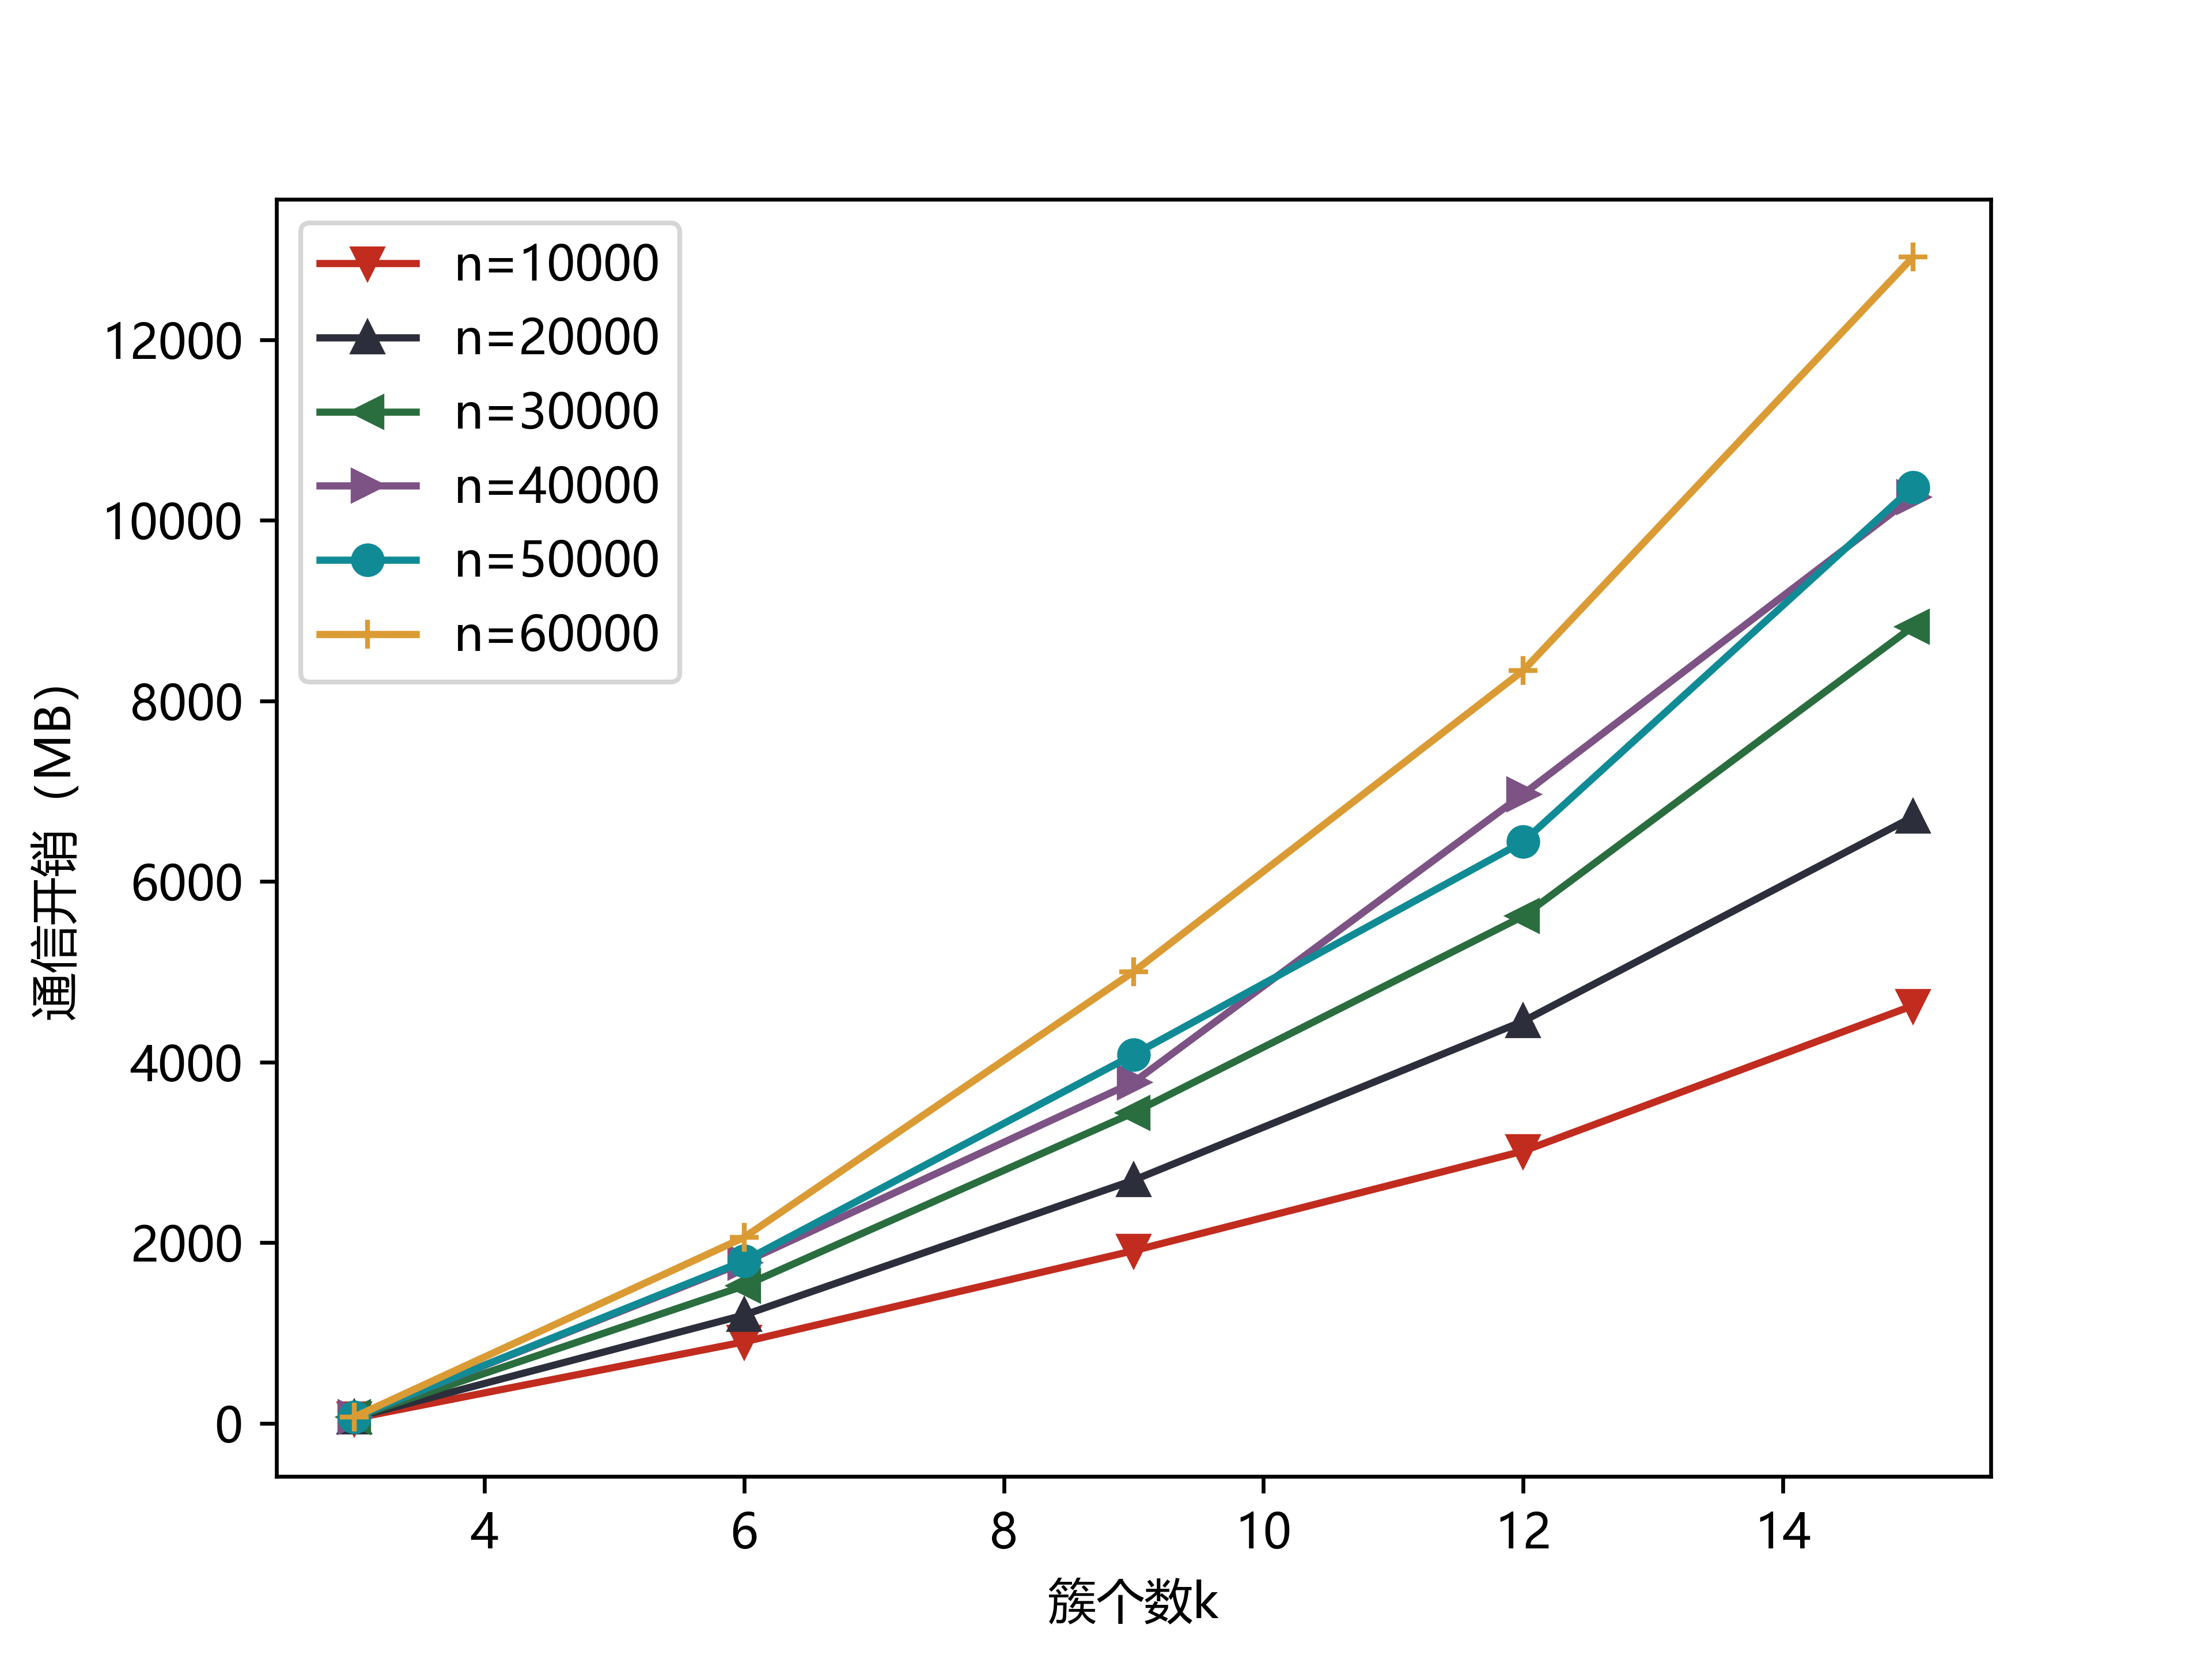
\includegraphics[width=\linewidth]{img/newk_comm.png}
		
	\end{minipage}
	\caption{簇个数$ k $对方案开销的影响}
	\label{f7}
\end{figure}

对于图\ref{f7},这里固定$ m=5,T=20 $,变化簇个数$ k $的大小,观察计算和通信开销的变化趋势。
计算开销和通信开销随着簇个数$ k $的增加而呈现近似线性变化趋势,从数据跨度角度进行分析,当$ k $较小时,不同数据集之间的开销差异较小;当$ k $较大时,不同数据集之间的开销差异显著增加,以计算开销为例,当k=15时,n=10000的数据集与n=60000的数据集之间的用时差异约为4000s。实验结果符合对于方案的分析,随着簇个数$ k $的增加,安全过滤算法中安全比较以及安全极值协议的运行次数也会显著增加。

通过分析实验结果,本文提出的方案兼具高效与安全性,并且能够适应大型数据集。与研究\cite{wu2020secure,rong2017privacy}相比,本文的方案在$ k $较大时,实验表现更好。基于Kd-tree的改进K-means算法允许减少大量冗余计算,进一步加速聚类过程,此外,SIMD操作可以很轻松被引入方案来提升效率。

\section{本章小结}
\label{s3-xiaojie}
% 简述存在的问题
隐私保护K-means聚类方案的研究通常难以兼具效率与安全性,实现完全隐私保护的方案耗时通常难以接受\cite{jaschke2019unsupervised},高效的方案则可能存在泄露隐私的风险\cite{wu2020secure}。过去研究常用到的密码学工具为秘密共享\cite{mohassel2019practical}和同态加密\cite{jaschke2019unsupervised}\cite{wu2020secure},二者各有优缺点。秘密共享技术进行加法和乘法运算较快,但是通信开销较大,而同态加密则计算开销较大,通信开销较小。

% 本文方案的贡献
为了能够设计兼具安全与高效的隐私保护K-means聚类方案,本文在秘密共享的基础上,提出了一个基于Kd-tree的隐私保护外包K-means聚类方案。方案利用了Kd-tree数据结构来减少冗余计算,提升聚类效率,同时保证聚类的正确性。此外,提出了基于秘密共享设计了一系列隐私保护的计算协议,这些协议独立于整个方案,可以灵活的用于其他各种基于秘密共享的隐私保护方案中。实验结果证明,本文的方案在保证聚类结果正确的基础上,保护了数据的隐私安全,减少了计算和通信开销,为用户提供了一种实际可行的外包聚类方案。

% 引出下一个点
然而,聚类通常是对海量数据进行分析挖掘,数据量级可以达到亿万级别。在该场景下,即便是目前最高效的隐私保护聚类方案所需时间也是不可接受的。因此需要探索新的方案设计方向,即近似的隐私保护方案。机器学习对于计算的精度要求通常较宽松,因此可以考虑通过设计近似安全计算协议来简化计算过程,提升效率。